\documentclass[ROIA,Unicode]{cedram}

\AtBeginDocument{\inputencoding{utf8}}
\usepackage[numbers,sort&compress]{natbib}
\usepackage{booktabs}
\usepackage{graphicx}
\usepackage{longtable}
\usepackage{tabularx}
\usepackage{xurl}
\usepackage{microtype}

\datereceived{2026-04-20}
\issueinfo{0}{0}{0}{2026}
\SetFirstPage{1}

\makeatletter
\def\@setdates{%
\vglue4mm
\rightline{\itshape\Small
\ifx\@empty\@datereceived\else\@setdatereceived\fi
\ifx\@empty\@daterevised\else\@setdaterevised\fi}}
\makeatother

\makeatletter
\AtBeginDocument{%
\@ifundefined{theHtable}{}{% 
\renewcommand{\theHtable}{\thesection.\arabic{table}}}%
\@ifundefined{theHfigure}{}{% 
\renewcommand{\theHfigure}{\thesection.\arabic{figure}}}%
}
\makeatother

\title[LLMs, social sciences and epidemiology]{LLMs, social sciences and epidemiology: integrating socio-behavioral profiles into a French contact-matrix pipeline}
\alttitle{LLM, SHS et épidémiologie : intégration de profils socio-comportementaux dans un pipeline français de matrices de contact}

\author{\firstname{Martin} \lastname{Collins}}
\address{Université Paris 1 Panthéon-Sorbonne, University Diploma in Data Science, Paris, France}
\email{martin.collins-academie@proton.me}

\keywords{contact matrices, large language models, social sciences, epidemiological modeling, France, socio-behavioral profiles}
\altkeywords{matrices de contact, grands modèles de langage, sciences humaines et sociales, modélisation épidémiologique, France, profils socio-comportementaux}

\subjclass{62P10, 68T07, 91D10}

\emergencystretch=2em

\begin{document}
\selectlanguage{english}

\begin{abstract}
Age-structured contact matrices are central to epidemic modeling, yet they compress social heterogeneity and rarely articulate how behavioral change should be reintroduced in a transparent way. The paper addresses a specific question: can a socio-behavioral LLM layer enrich a French contact-matrix pipeline without hiding its assumptions behind black-box claims?

We therefore develop an incremental protocol in four stages. First, we compare a minimal demographic rescaling with a contextual baseline structured by home, school, work and community contacts, then optimize this baseline on COMES-F. Second, we add a lightweight temporal behavioral layer calibrated on French CoviPrev and SocialCov series. Third, we introduce 18 explicit socio-demographic profiles and a first campaign of real LLM generations, using Claude Sonnet 4.6, to recover regime ordering and social heterogeneity. Fourth, we make the LLM block more central by turning it into a structured social-science mediation layer, iteratively refined through experiments exp007, exp008 and exp009, with a final campaign on Claude Haiku 4.5 and a revised mobility-oriented prompt.

The static baseline remains useful, but the main result now lies in the LLM block. The first campaign already recovers plausible differences in responsiveness between white-collar and agricultural profiles. More importantly, the exp007 to exp009 sequence shows that the main bottleneck was not the SHS-LLM hypothesis itself, but the calibration of the latent mobility variable. In the final exp009 configuration, the LLM layer outperforms the heuristic benchmark on both mobility and prevention, with a mobility MAE of 0.0219 versus 0.0935, a mobility correlation of 0.989 versus 0.863, and a prevention MAE of 0.0685 versus 0.1409. The contribution is therefore not a claim that LLMs replace survey data, but a transparent and auditable protocol showing how they can be inserted as socio-behavioral mediators between public policy regimes, named social profiles and diffusion-relevant contact modifiers.
\end{abstract}

\begin{altabstract}
Les matrices de contact par âge sont centrales en modélisation épidémiologique, mais elles écrasent souvent une partie des différences sociales de comportement et explicitent rarement la manière de les réintroduire sans opacifier le modèle. Le présent article s'organise autour d'une question précise : une couche LLM socio-comportementale peut-elle enrichir un pipeline français de matrices de contact tout en gardant ses hypothèses visibles et auditables ?

Pour y répondre, nous développons un protocole incrémental en quatre étapes. D'abord, nous comparons une repondération démographique minimale à un socle contextuel structuré par domicile, école, travail et communauté, puis nous optimisons ce socle sur COMES-F. Ensuite, nous ajoutons une couche comportementale temporelle légère calibrée sur les séries françaises CoviPrev et SocialCov. Puis nous introduisons 18 profils socio-démographiques explicites et une première campagne de générations réelles par LLM, avec Claude Sonnet 4.6, afin de restituer l'ordre des régimes sanitaires et une hétérogénéité sociale plausible. Enfin, nous rendons le bloc LLM plus central en le reformulant comme couche de médiation SHS structurée, raffinée itérativement au fil des expériences exp007, exp008 et exp009, avec une campagne finale sur Claude Haiku 4.5 et un prompt révisé centré sur la mobilité.

Le socle statique reste utile, mais le résultat principal se situe désormais dans le bloc LLM. La première campagne fait déjà apparaître des écarts plausibles de réactivité entre profils cadres et profils agricoles. Surtout, la séquence exp007 à exp009 montre que le principal verrou n'était pas l'hypothèse SHS-LLM en elle-même, mais le calibrage de la variable latente de mobilité. Dans la configuration finale exp009, la couche LLM surpasse la référence heuristique à la fois sur la mobilité et sur la prévention, avec une MAE mobilité de 0,0219 contre 0,0935, une corrélation mobilité de 0,989 contre 0,863, et une MAE prévention de 0,0685 contre 0,1409. La contribution n'est donc pas de prétendre que les LLM remplacent les enquêtes, mais de proposer un protocole transparent et auditable montrant comment les insérer comme médiateurs socio-comportementaux entre régimes de politique publique, profils sociaux nommés et modificateurs de contact utiles à la diffusion épidémique.
\end{altabstract}

\maketitle

\section{Introduction}
This study was conducted as part of the University Diploma in Data Science at Université Paris 1 Panthéon-Sorbonne. Its core ambition is the progressive integration of an explicit socio-behavioral mediator between public policy regimes, named social profiles and contact modifiers relevant to epidemic modeling.

Age-structured contact matrices play a decisive role in transmission models because they quantify how age groups meet. Yet, in their standard form, they remain poorly suited to representing unequal room for maneuver across social groups during a health crisis. Between a national aggregated matrix and a heavy agent-based simulation, there is often no intermediate layer able to make explicit social profiles, mobility constraints, differences in institutional trust and unequal capacities to comply with preventive measures. Documenting that missing methodological layer is the central purpose of this paper.

The French case is a useful setting for such an attempt. COMES-F provides a robust empirical anchor for contact structure \citep{beraud2015french}, while CoviPrev, SocialCov and Google Mobility document temporal transformations of behavior during the pandemic \citep{coviprev2021,socialcov2024,googlemobility2022}. None of these datasets, however, directly articulates contact structure, social position and behavioral response. Our hypothesis is that a bounded, profiled and audited LLM layer can play that mediating role, provided that it remains strictly constrained, compared against explicit baselines, and interpreted as a structured scenario instrument rather than a direct measure of true behavior.

The manuscript therefore follows a trajectory of increasing complexity. We first establish a transparent static baseline, then add a calibratable temporal layer, and only afterwards make the LLM block central to the analysis. This trajectory matters scientifically because it separates what comes from a better structural baseline, what comes from a still fragile temporal calibration, and what stems from the introduction of socio-behavioral mediation through an LLM. Recent iterations of the project play a substantive role here. A first campaign based on real calls to Claude Sonnet 4.6 showed that it was possible to recover a plausible hierarchy of policy regimes and socially differentiated responsiveness. A second series of experiments, exp007 to exp009, then revealed that the major difficulty lay less in the SHS-LLM idea itself than in the framing of the latent \emph{mobility\_reduction} variable. The final exp009 version, executed with Claude Haiku 4.5 and a revised prompt protocol, specifically addresses that issue.

The paper pursues four objectives. First, to establish a reproducible French baseline for synthetic contact matrices. Second, to show what a lightweight behavioral layer does and does not add once the problem becomes time-varying. Third, to test whether explicit socio-demographic profiles allow an LLM to produce plausible social differences and plausible ordering across public-health regimes. Fourth, to document honestly how the performance of the LLM block depends on the mediation protocol, the prompt and the model. The main contribution is therefore no longer only an incremental pipeline. It is the explicit, traceable and contestable integration of an SHS/LLM layer into a French epidemiological modeling chain.

\section{Related work}
Contact surveys remain the most convincing starting point for describing intergenerational mixing relevant to public health. POLYMOD played a foundational role by demonstrating the robustness of several contact motifs, especially age assortativity and the importance of daily contexts \citep{mossong2008social}. For France, COMES-F provided a decisive empirical anchor by documenting reported contacts, their variation across the calendar and the need to correct reciprocity biases \citep{beraud2015french}. These studies are more than comparison points. They also define the minimal structural properties that a credible synthetic matrix should recover, at least approximately.

A second family of studies aims not so much to measure contacts directly as to project them into countries or regions without dedicated surveys. The matrices of Prem and colleagues have become a major reference by combining existing surveys, demographic structure, school organization and labor participation in order to produce synthetic matrices with broad geographical coverage \citep{prem2017projecting,prem2021projecting}. This approach is extremely valuable, and we retain its core intuition: a decomposition by contexts improves transferability. Our objective is narrower, however. We do not attempt to rebuild an international hierarchical model. We instead examine what can be obtained in a lighter French setting where assumptions remain immediately inspectable.

A third line of research pushes synthesis much further by constructing rich artificial populations from socio-demographic microdata and explicit mechanisms assigning individuals to households, schools or workplaces \citep{mistry2021inferring}. These pipelines offer much stronger structural realism and open the door to fine-grained analyses, especially at subnational level. They also require more data, more modeling choices and a heavier validation chain. Our work stands upstream of that ambition. It borrows the intuition of home, school, work and other components, simplifies social structure substantially, and leaves full synthetic-population generation, detailed temporal dynamics and regional modeling outside the present scope.

Since 2023, a distinct literature has explored the use of large language models as social simulators, generative agents or stylized economic agents \citep{park2023generative,argyle2023out,horton2023homo}. This literature shows that an LLM can recover plausible action hierarchies when grounded in explicit roles or constraints. It also makes clear that such systems remain highly dependent on profile formulation, prompt variables and model-specific biases \citep{weidinger2022taxonomy,bender2021stochastic}. Our work takes up this exploratory intuition in a more bounded setting: named synthetic profiles, constrained JSON outputs, archived caches and comparison with aggregated French series rather than observed individual behavior.

Finally, recent work on France has made it clear that a contact matrix is not a static object. Repeated surveys and open datasets on preventive behavior show how strongly contact patterns and barrier measures changed across periods and policy constraints \citep{soussand2025socialcov,socialcov2024,coviprev2021}. This literature is essential for thinking about time-dependent effective matrices. It does not replace a clearly identified static base. It therefore remains useful to establish a simple, reproducible and well-evaluated French baseline before adding more ambitious temporal mechanisms.

\section{Methodology}
The protocol relies on a common discretization with $K=17$ age classes covering the interval $[0,85]$ years on a regular grid. A contact matrix is denoted $M \in \mathbb{R}_{+}^{K\times K}$, where entry $M_{ij}$ represents the average contact intensity from group $i$ to group $j$. The project is built as a four-layer incremental chain: static baseline, temporal layer, socio-behavioral profiles, then SHS mediation by LLMs. This progression is not a mere development history. It is the methodological device itself, because each layer becomes the control for the next one.

The inputs remain deliberately limited. We use an age-population vector $\mathbf{p}=(p_1,\dots,p_K)$, strictly positive, together with four initial components corresponding to home, school, work and other community interactions. In the first experiments these components were first produced by a deterministic synthetic generator, then confronted with real COMES-F data for structural validation and contextual optimization. They are symmetrized before use so that directional artefacts do not blur the interpretation of baseline models.

The first reference model, called \emph{demographic rescaling}, starts from an aggregated template matrix
\[
T = H + S + W + O,
\]
where $H$, $S$, $W$ and $O$ denote the \emph{home}, \emph{school}, \emph{work} and \emph{other} components, respectively. Each row of $T$ is first normalized, then reweighted by the demographic mass of the emitting group:
\[
\widehat{M}^{\mathrm{demo}}_{ij} = \frac{T_{ij}}{\sum_{\ell=1}^{K} T_{i\ell}}\, p_i.
\]
This model answers a simple question: what is gained if one only adapts demographic exposure, without modifying the topology of contacts?

The second model introduces a more interpretable structure. Four components are built separately and then added:
\[
\widehat{M}^{\mathrm{hh}} = M^{\mathrm{home}} + M^{\mathrm{school}} + M^{\mathrm{work}} + M^{\mathrm{other}}.
\]
The \emph{hh} superscript refers here to the context-structured baseline. The home component combines a co-residence diagonal, parent-child bands, a spousal proximity term and a weaker grandparent-child interaction. The school component concentrates around school ages. The work component spreads over working ages. A low-amplitude community component finally adds a nonspecific mixing background. Each term is weighted by a demographic exposure factor of the form $\sqrt{p_i p_j}$ in order to preserve a simple reading of the contribution of group sizes.

A first extension directly optimizes the home, school, work and other weights on COMES-F. A second adds a lightweight temporal behavioral layer that is bounded and calibratable on French data. Up to this point the logic remains classical: establish a better static base, then test a more flexible temporal dynamic. The third layer then introduces a clearly central SHS/LLM component.

This extra layer does not attempt to reconstruct a full synthetic population. It rests on 18 profile-situations spanning ten broad French socio-demographic positions: manual workers, employees, white-collar professionals, intermediate professions, retirees, students, inactive adults, craftspeople or shopkeepers, farmers and unemployed adults. Each profile combines a dominant age, a residential configuration, a degree of mobility constraint, a level of digital flexibility and a cautious proxy for institutional trust. The goal is not to imitate observed individuals, but to define an intermediate level between national aggregated series and heavy agent-based modeling. Profile construction combines the French socio-professional classification \citep{insee2016pcs}, plausible household structures \citep{insee2021menages}, differentiated opportunities for remote work \citep{dares2024teletravail} and behavioral gradients visible in CoviPrev \citep{coviprev2021}. Table~\ref{tab:profiles} summarizes these profiles.

The LLM block then evolved in two phases. In the first campaign retained in the manuscript, profiles are submitted to a behavioral generator with constrained JSON outputs and directly produce scores for mobility, mask use, distancing, risk perception and trust. This campaign relies on real calls to Claude Sonnet 4.6 and primarily tests two properties: ordering of policy regimes and plausibility of social differences across profiles. In the second phase, conducted through exp007, exp008 and exp009, the LLM is no longer used only as a direct generator of final scores. It becomes a structured SHS mediator: it produces latent variables such as adherence, risk perception, trust, mobility reduction, policy fatigue or compliance capacity, which are then projected into the calibrated behavioral layer in order to obtain contact and transmission modifiers more directly connected to the epidemiological pipeline.

This second phase matters methodologically because it documents the steps taken. Exp007 constitutes a first version of the SHS mediator. Prevention signal is already better than the heuristic, but the mobility variable remains poorly calibrated. Exp008 then plays the role of a diagnostic experiment: by explicitly anchoring the mobility component, it shows that a large part of the gap does not come from a structural impossibility of the SHS/LLM block, but from the framing of the \emph{mobility\_reduction} variable. Exp009 finally corresponds to the retained final campaign: the same mediation architecture, a revised prompt centered on mobility, and a final execution on Claude Haiku 4.5. The final protocol keeps constrained JSON outputs, systematic archiving of generations and explicit comparison with a heuristic baseline. We therefore interpret the LLM block as a bounded socio-behavioral scenario instrument rather than as identification of real individual behavior.

\section{Experiments}
The main evaluation follows four families of experiments. Experiments \texttt{exp001\_real} and \texttt{exp004} concern the static baseline and its optimization on COMES-F. Experiment \texttt{exp003\_time\_series\_behavioral} evaluates the temporal layer on CoviPrev and SocialCov. Experiment \texttt{exp006\_llm\_agents} constitutes the first explicit-profile LLM campaign. Finally, the \texttt{exp007}, \texttt{exp008} and \texttt{exp009} sequence places SHS/LLM mediation at the center of the evaluation.

The reproducibility policy remains strict. A single seed, fixed at 2026 in the deterministic blocks, drives the synthetic phases of the pipeline, while structural and temporal validations rely on COMES-F, CoviPrev, SocialCov and Google Mobility. Archived LLM campaigns preserve their JSON outputs, aggregations and metadata necessary to reproduce the retained tables and figures exactly. This traceability makes it possible to distinguish clearly between fully deterministic blocks and blocks that depend on archived generations.

Four families of indicators are reported. Mean absolute error (MAE) captures the average gap between reference and prediction. Frobenius distance measures global matrix misfit. Age assortativity is summarized through strict diagonal mass and its local diffusion. Finally, the temporal block and the LLM block use correlations, directional agreement and MAE comparisons against heuristic baselines. These metrics do not exhaust the validity of a social simulation, but they are well suited to the logic adopted here: documenting what each layer improves, and what it still fails to explain.

We deliberately retain the intermediate steps of the exp007 to exp009 sequence. They are not narrated as a simple trial-and-error story, but because they change the scientific status of the final result. In this block, useful information is not only that one final number looks good. It is understanding why a first formulation of the mediator fails, how a focused diagnostic isolates the problematic variable, and how a final campaign, on another LLM and with a revised prompt, turns a fragile signal into a methodologically defensible result.

\section{Results}
\subsection{The static baseline remains the necessary control}
The two reference models produce strongly contrasting profiles. Demographic rescaling preserves part of the template matrix shape, but diverges sharply from the empirical reference once absolute magnitudes are considered. By contrast, the context-structured model reaches a very low error level and provides the anchor required for the rest of the paper. In this version of the article, that block is no longer presented as the main contribution, but as the indispensable control without which the temporal and LLM extensions would remain difficult to interpret.

\begin{table}[ht]
    \centering
    \small
    \caption{Quantitative comparison of static baseline models. MAE and Frobenius distance are expressed as average contact intensity per cell. Diagonal share and reciprocity gap are unit-free quantities.}
    \resizebox{\linewidth}{!}{%
    \begin{tabular}{lrrrr}
        \toprule
        Model & MAE (a.u.) & Frobenius distance (a.u.) & Diagonal share & Reciprocity gap \\
        \midrule
        Demographic rescaling & 6.48 & 198.42 & 0.240 & 4.22 \\
        Household heuristic & 0.35 & 8.82 & 0.139 & 0.00 \\
        Household optimization & 0.27 & 7.17 & 0.163 & 0.00 \\
        \bottomrule
    \end{tabular}%
    }
\end{table}

Direct optimization of the home, school, work and other weights on COMES-F reduces MAE from 0.35 to 0.27, a relative gain of about 23.8\,\%, while preserving an interpretable reading of the components. This remains important for what follows: the LLM block is not plugged into an arbitrary base, but into a static baseline that has already been audited and tightened.

Figures \ref{fig:heatmaps} to \ref{fig:assortativity} confirm that reading. They show the visual proximity between the COMES-F reference, the heuristic household model and its optimized variant, as well as the clearer mismatch of the demographic model on intensities and symmetry. To preserve comparability across panels and the readability of low-intensity values, the matrix comparison is presented on a common logarithmic scale.

\begin{figure}[ht]
    \centering
    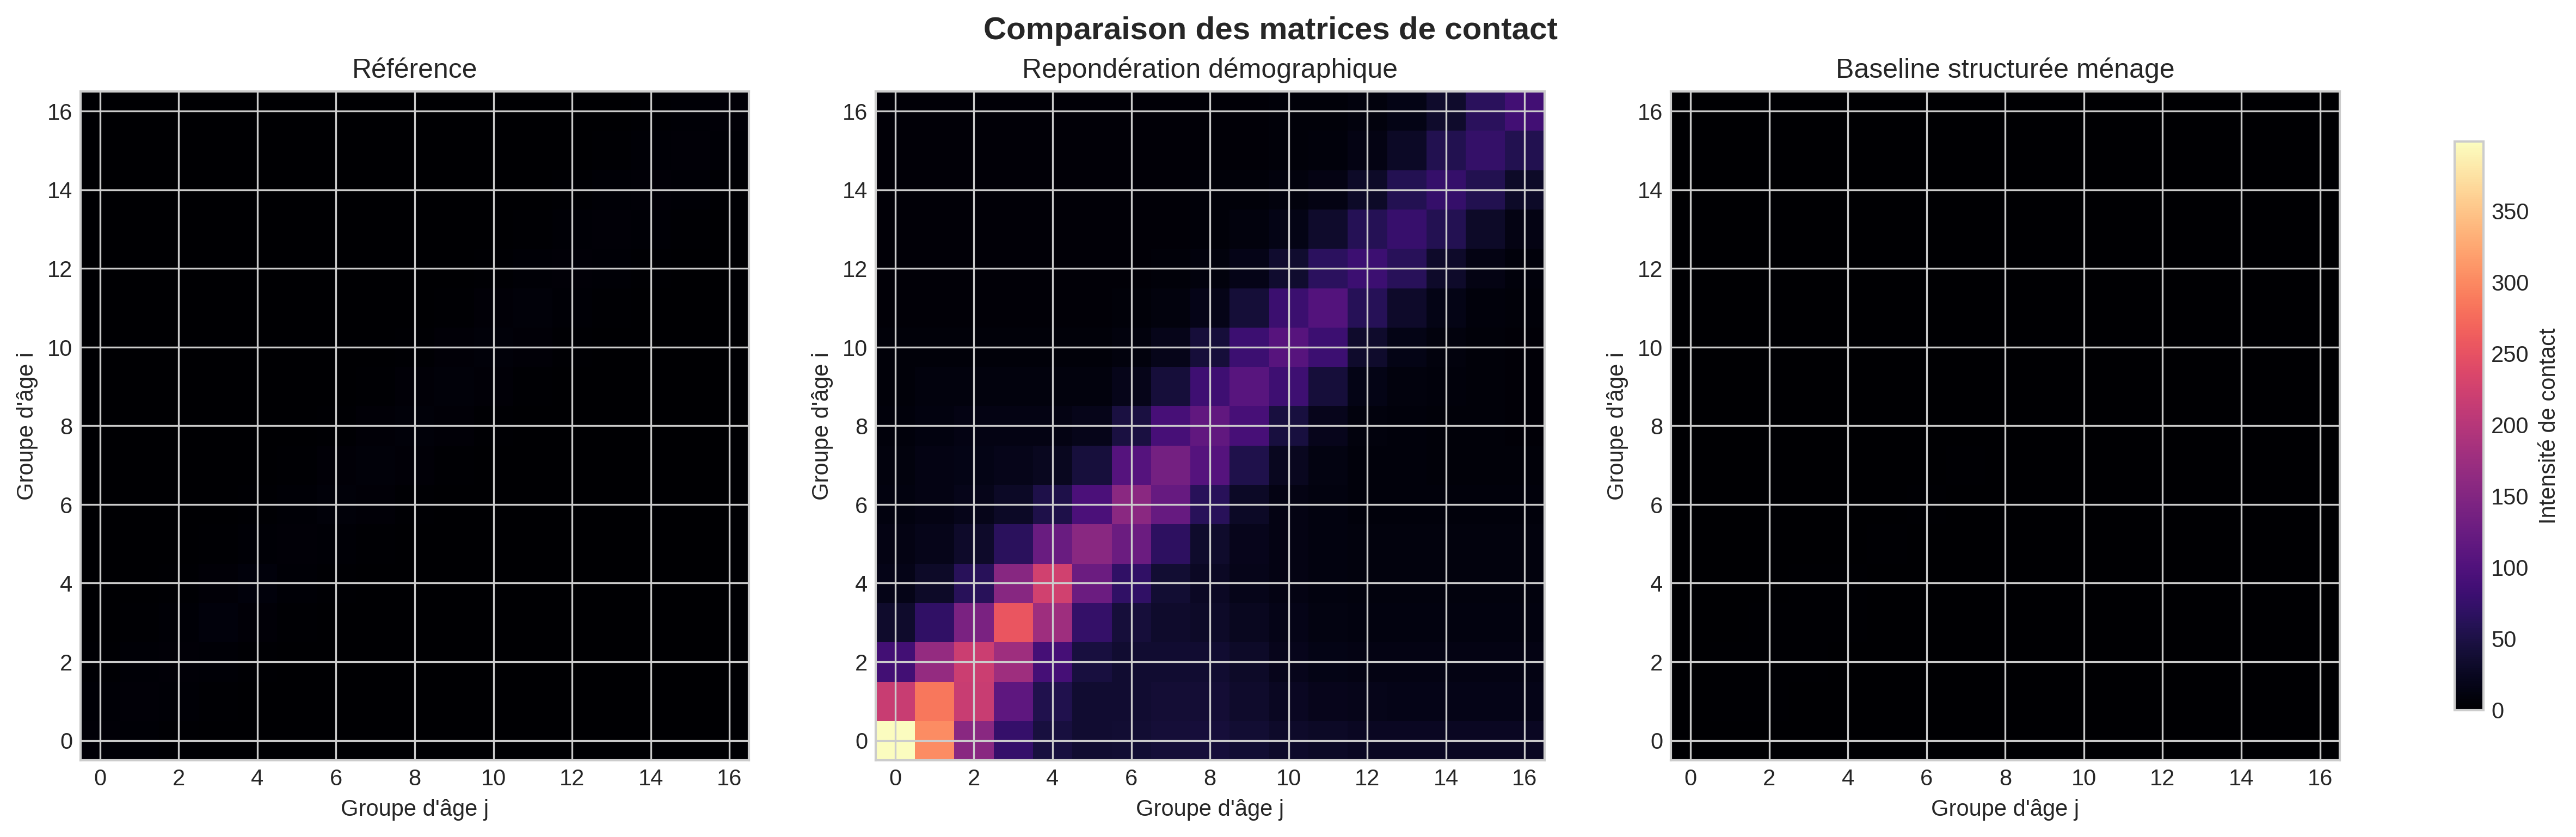
\includegraphics[width=0.98\textwidth]{figures/exp001_heatmaps.png}
    \caption{Visual comparison between the COMES-F reference, demographic rescaling, the heuristic household model and its optimized version. A common logarithmic scale is used to preserve comparability across panels without flattening low intensities.}
    \label{fig:heatmaps}
\end{figure}

\begin{figure}[ht]
    \centering
    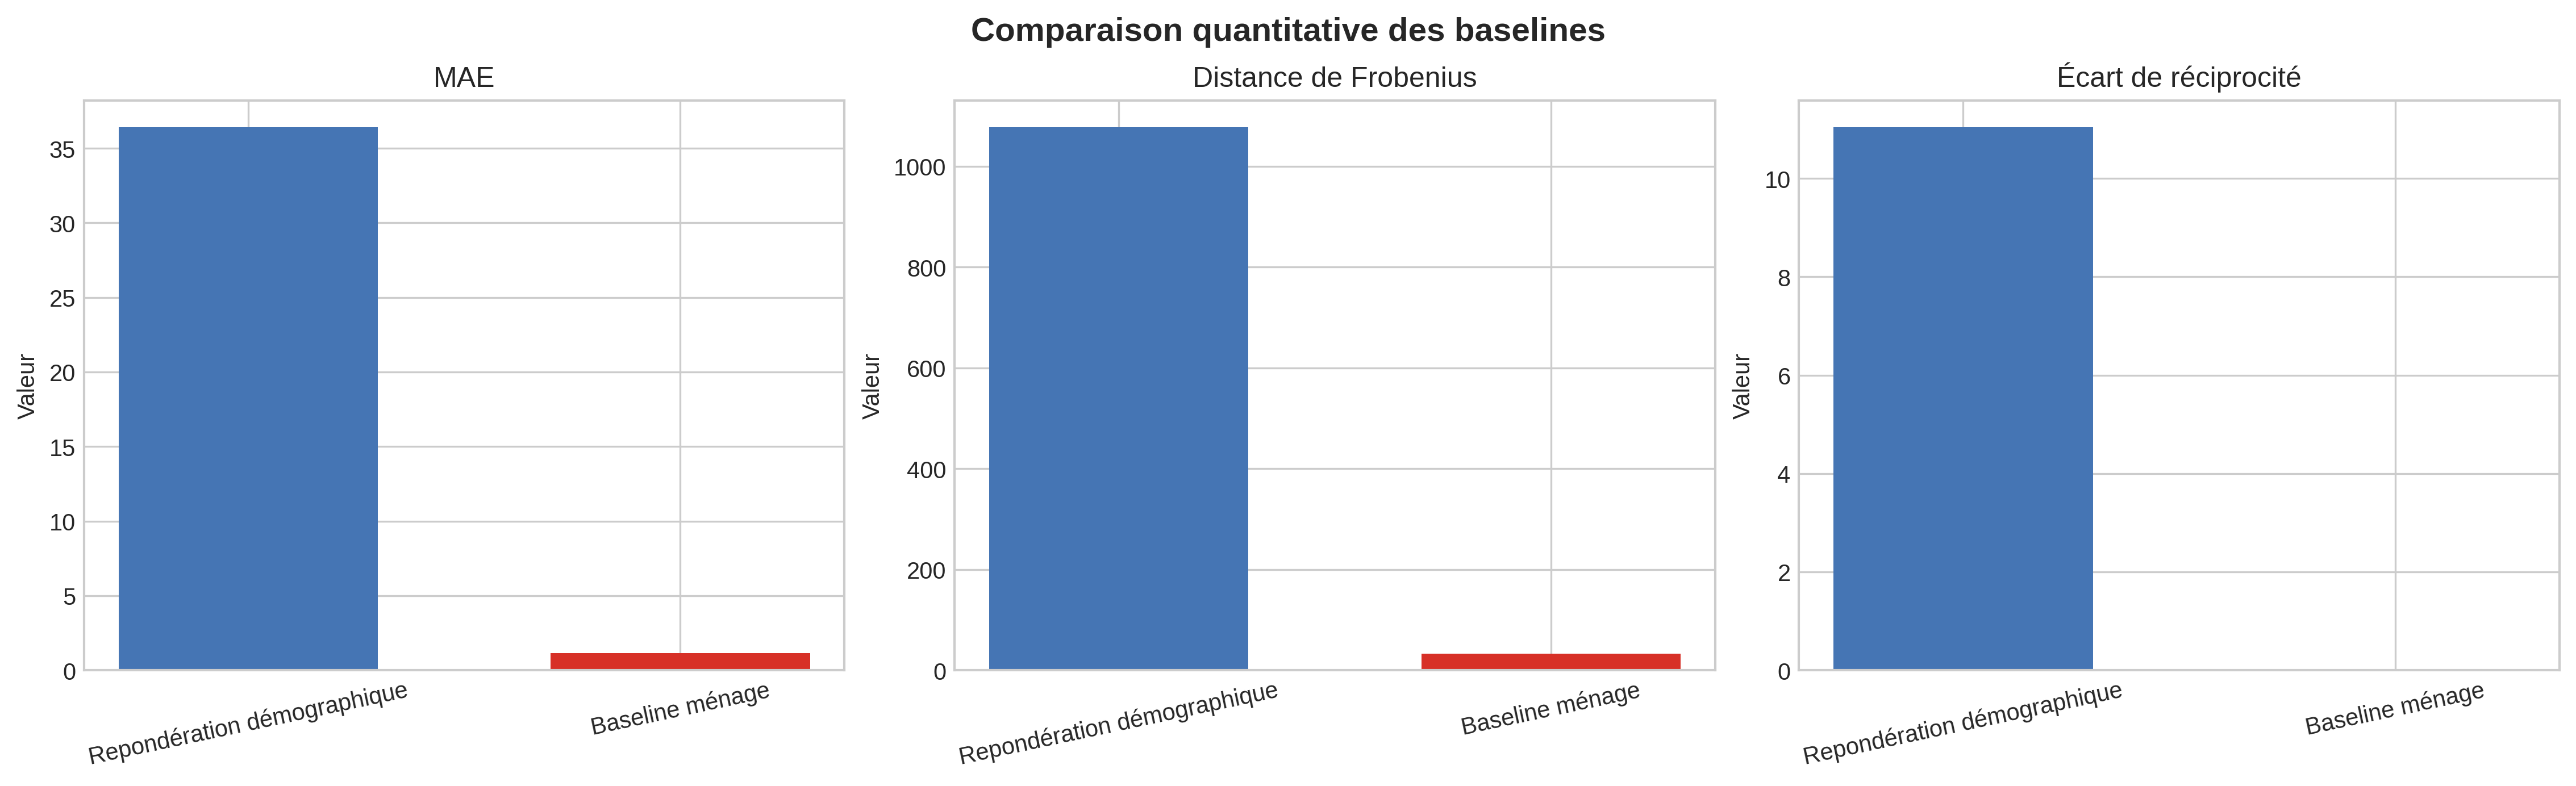
\includegraphics[width=0.98\textwidth]{figures/exp001_metrics.png}
    \caption{Comparison of the main error and structural-coherence metrics for the three static models.}
    \label{fig:metrics}
\end{figure}

\begin{figure}[ht]
    \centering
    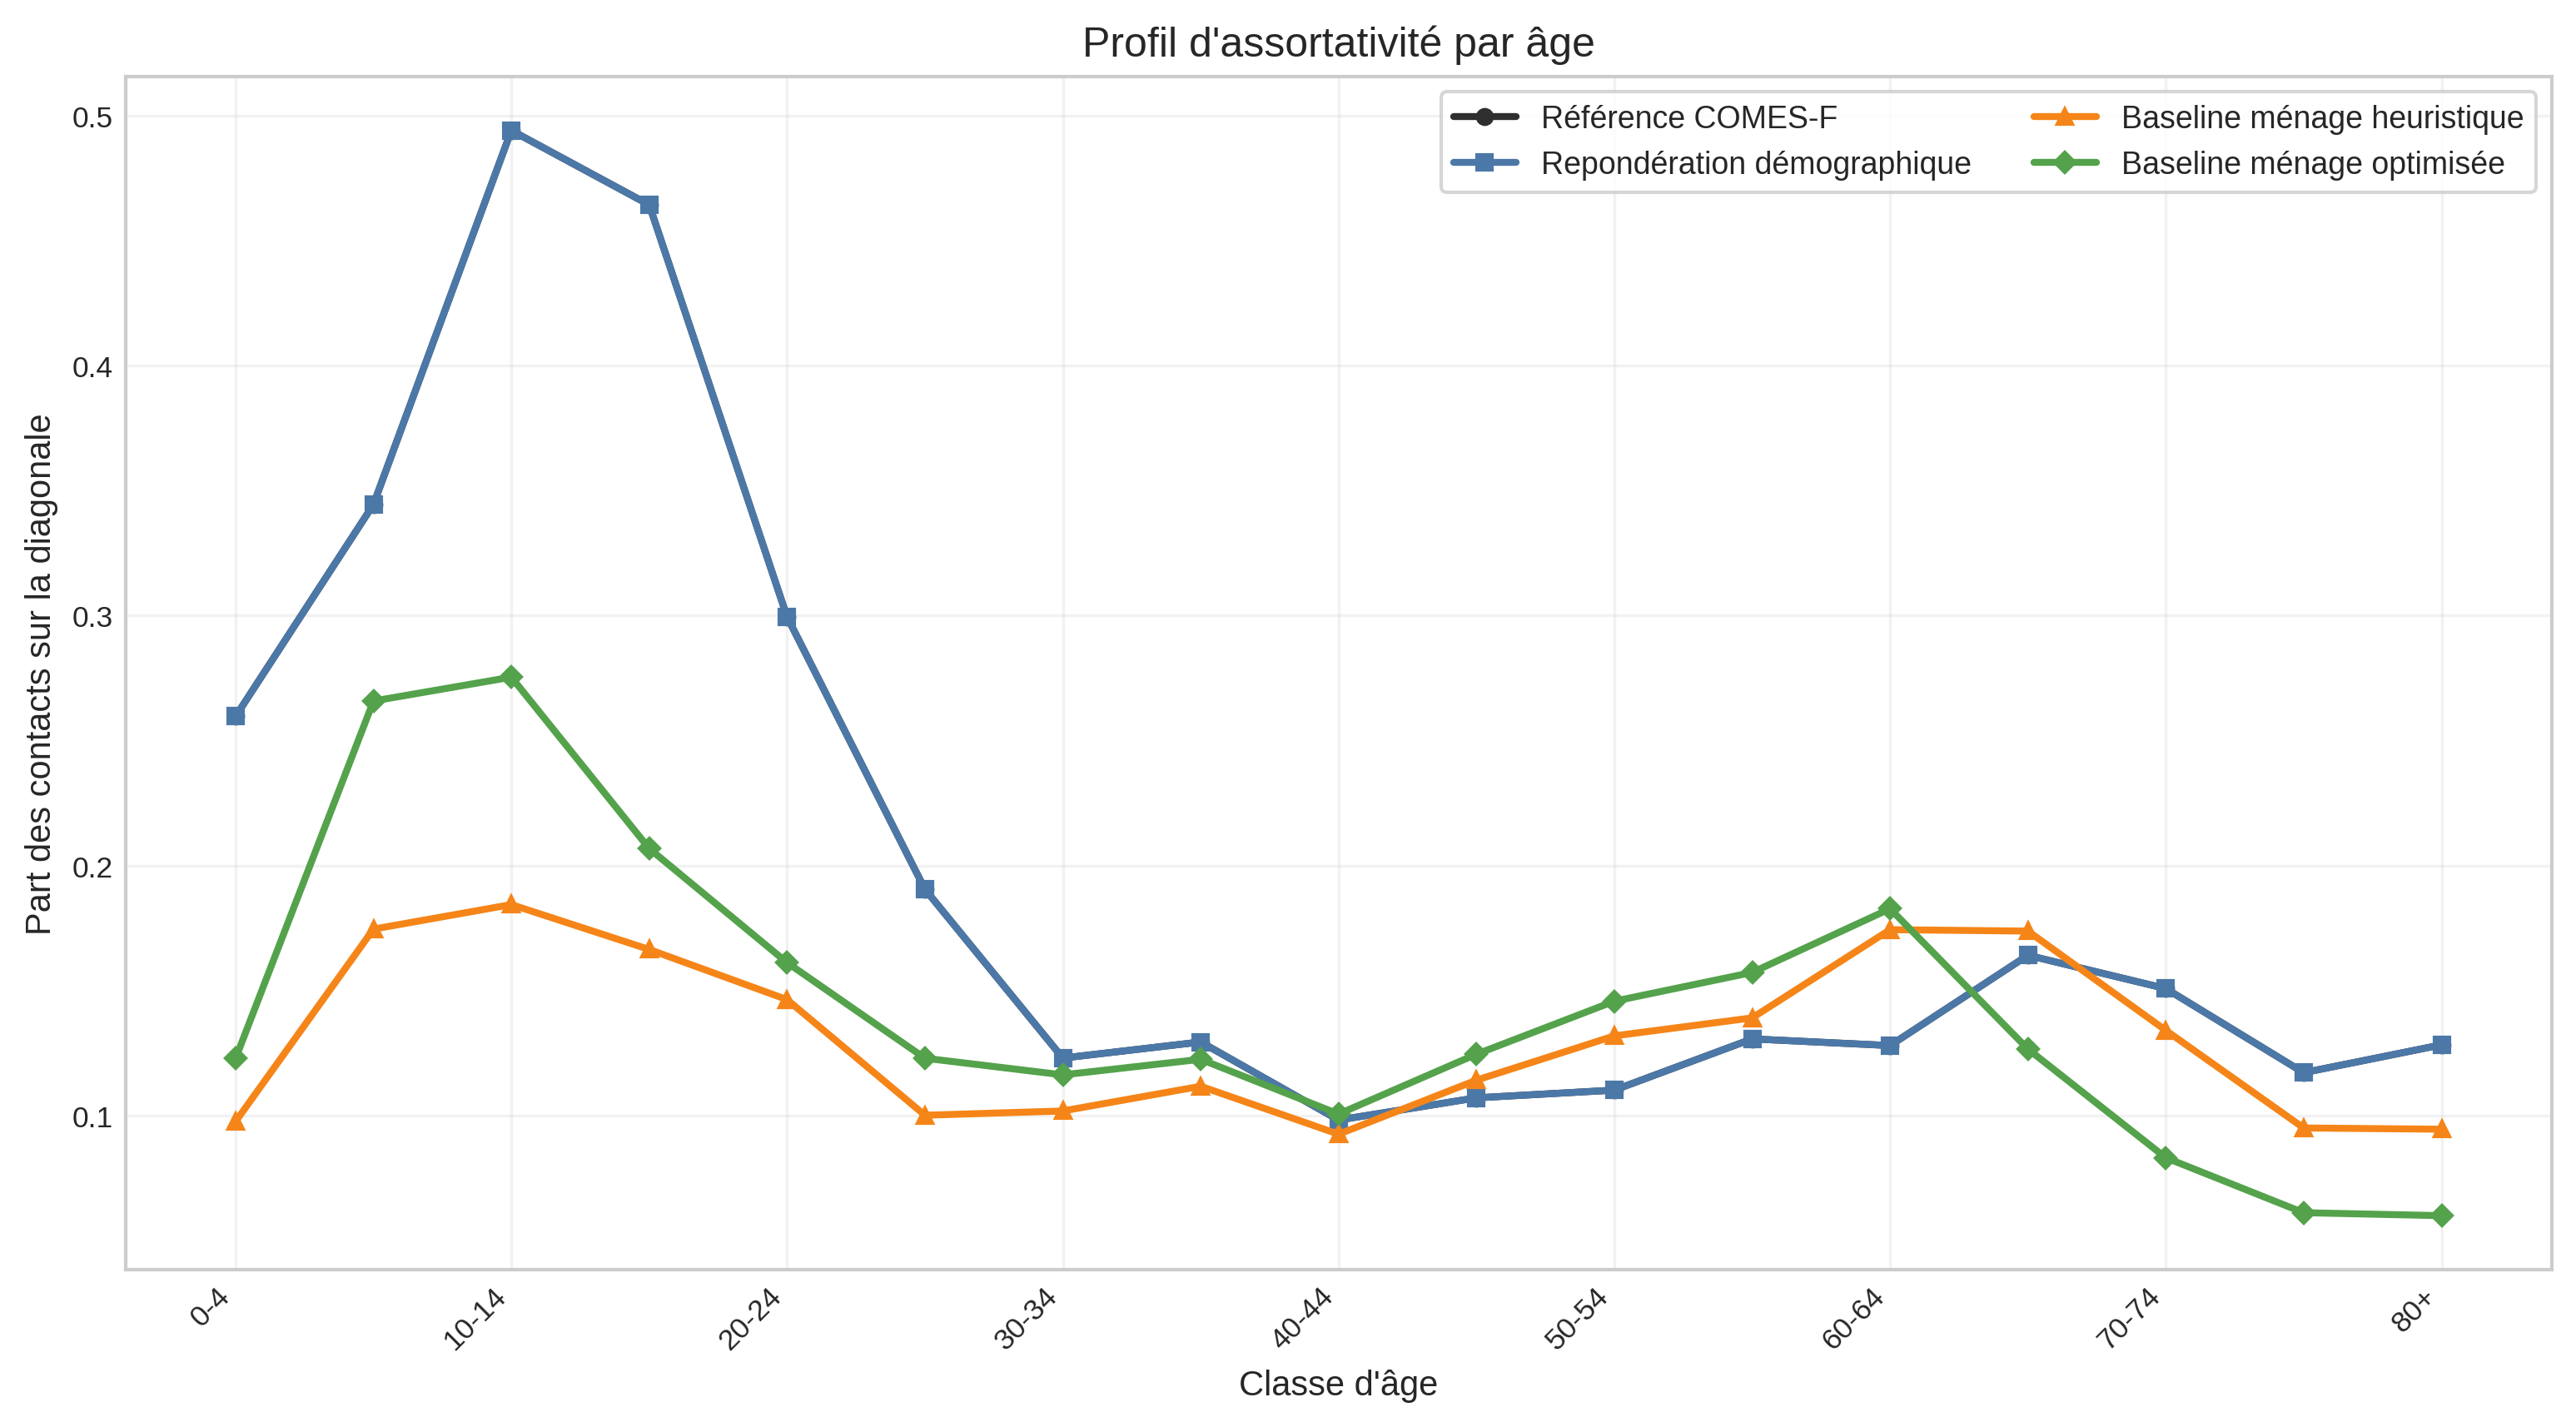
\includegraphics[width=0.80\textwidth]{figures/exp001_assortativity_profile.png}
    \caption{Age-assortativity profile for the empirical reference, demographic rescaling, the heuristic household model and its optimized version.}
    \label{fig:assortativity}
\end{figure}

\subsection{The temporal layer improves some series, but remains secondary}
Temporal validation quickly tempers the ambition of the manuscript. Once the exact SocialCov collection windows are realigned, the uncalibrated behavioral layer still reduces the MAE of the prevention index from 0.124 to 0.054 relative to a static reference, with directional agreement at 0.73. On SocialCov, however, fit remains difficult: MAE on relative contact changes reaches 0.265, versus 0.174 for the static reference, even though directional agreement rises from 0.00 to 0.40.

Chronological calibration improves training fit strongly, but remains fragile out of sample. For prevention, test MAE becomes 0.063, which is still better than the static reference but slightly worse than the uncalibrated behavioral layer. For SocialCov contacts, calibration improves test MAE modestly, from 0.305 to 0.274, while remaining clearly worse than the static reference at 0.121. The \path{remove_other_behavior} ablation brings test MAE down to 0.205 without degrading directional agreement, suggesting that part of the community component still absorbs policy ruptures too abruptly.

\begin{table}[ht]
    \centering
    \small
    \caption{Summary of temporal metrics after SocialCov realignment and calibration. All columns are unit-free scores between 0 and 1, except MAE, which remains expressed on the normalized scale of the series.}
    \begin{tabularx}{\linewidth}{>{\raggedright\arraybackslash}X r r r}
        \toprule
        Series and model & MAE & Directional agreement & Peak accuracy \\
        \midrule
        Prevention, uncalibrated behavioral & 0.054 & 0.73 & 0.50 \\
        Prevention, static & 0.124 & 0.00 & 0.50 \\
        Contacts, uncalibrated behavioral & 0.265 & 0.40 & 1.00 \\
        Contacts, static & 0.174 & 0.00 & 0.20 \\
        Prevention test, calibrated & 0.063 & 0.50 & 0.20 \\
        Contacts test, calibrated & 0.274 & 1.00 & 1.00 \\
        \bottomrule
    \end{tabularx}
\end{table}

Figures \ref{fig:exp003-prevention} and \ref{fig:exp003-contacts} summarize that asymmetry: the temporal signal is useful for documenting aggregated behavior, but it is not strong enough to carry the main contribution of the paper. It remains a useful intermediate layer, not the center of gravity of the manuscript.

\begin{figure}[ht]
    \centering
    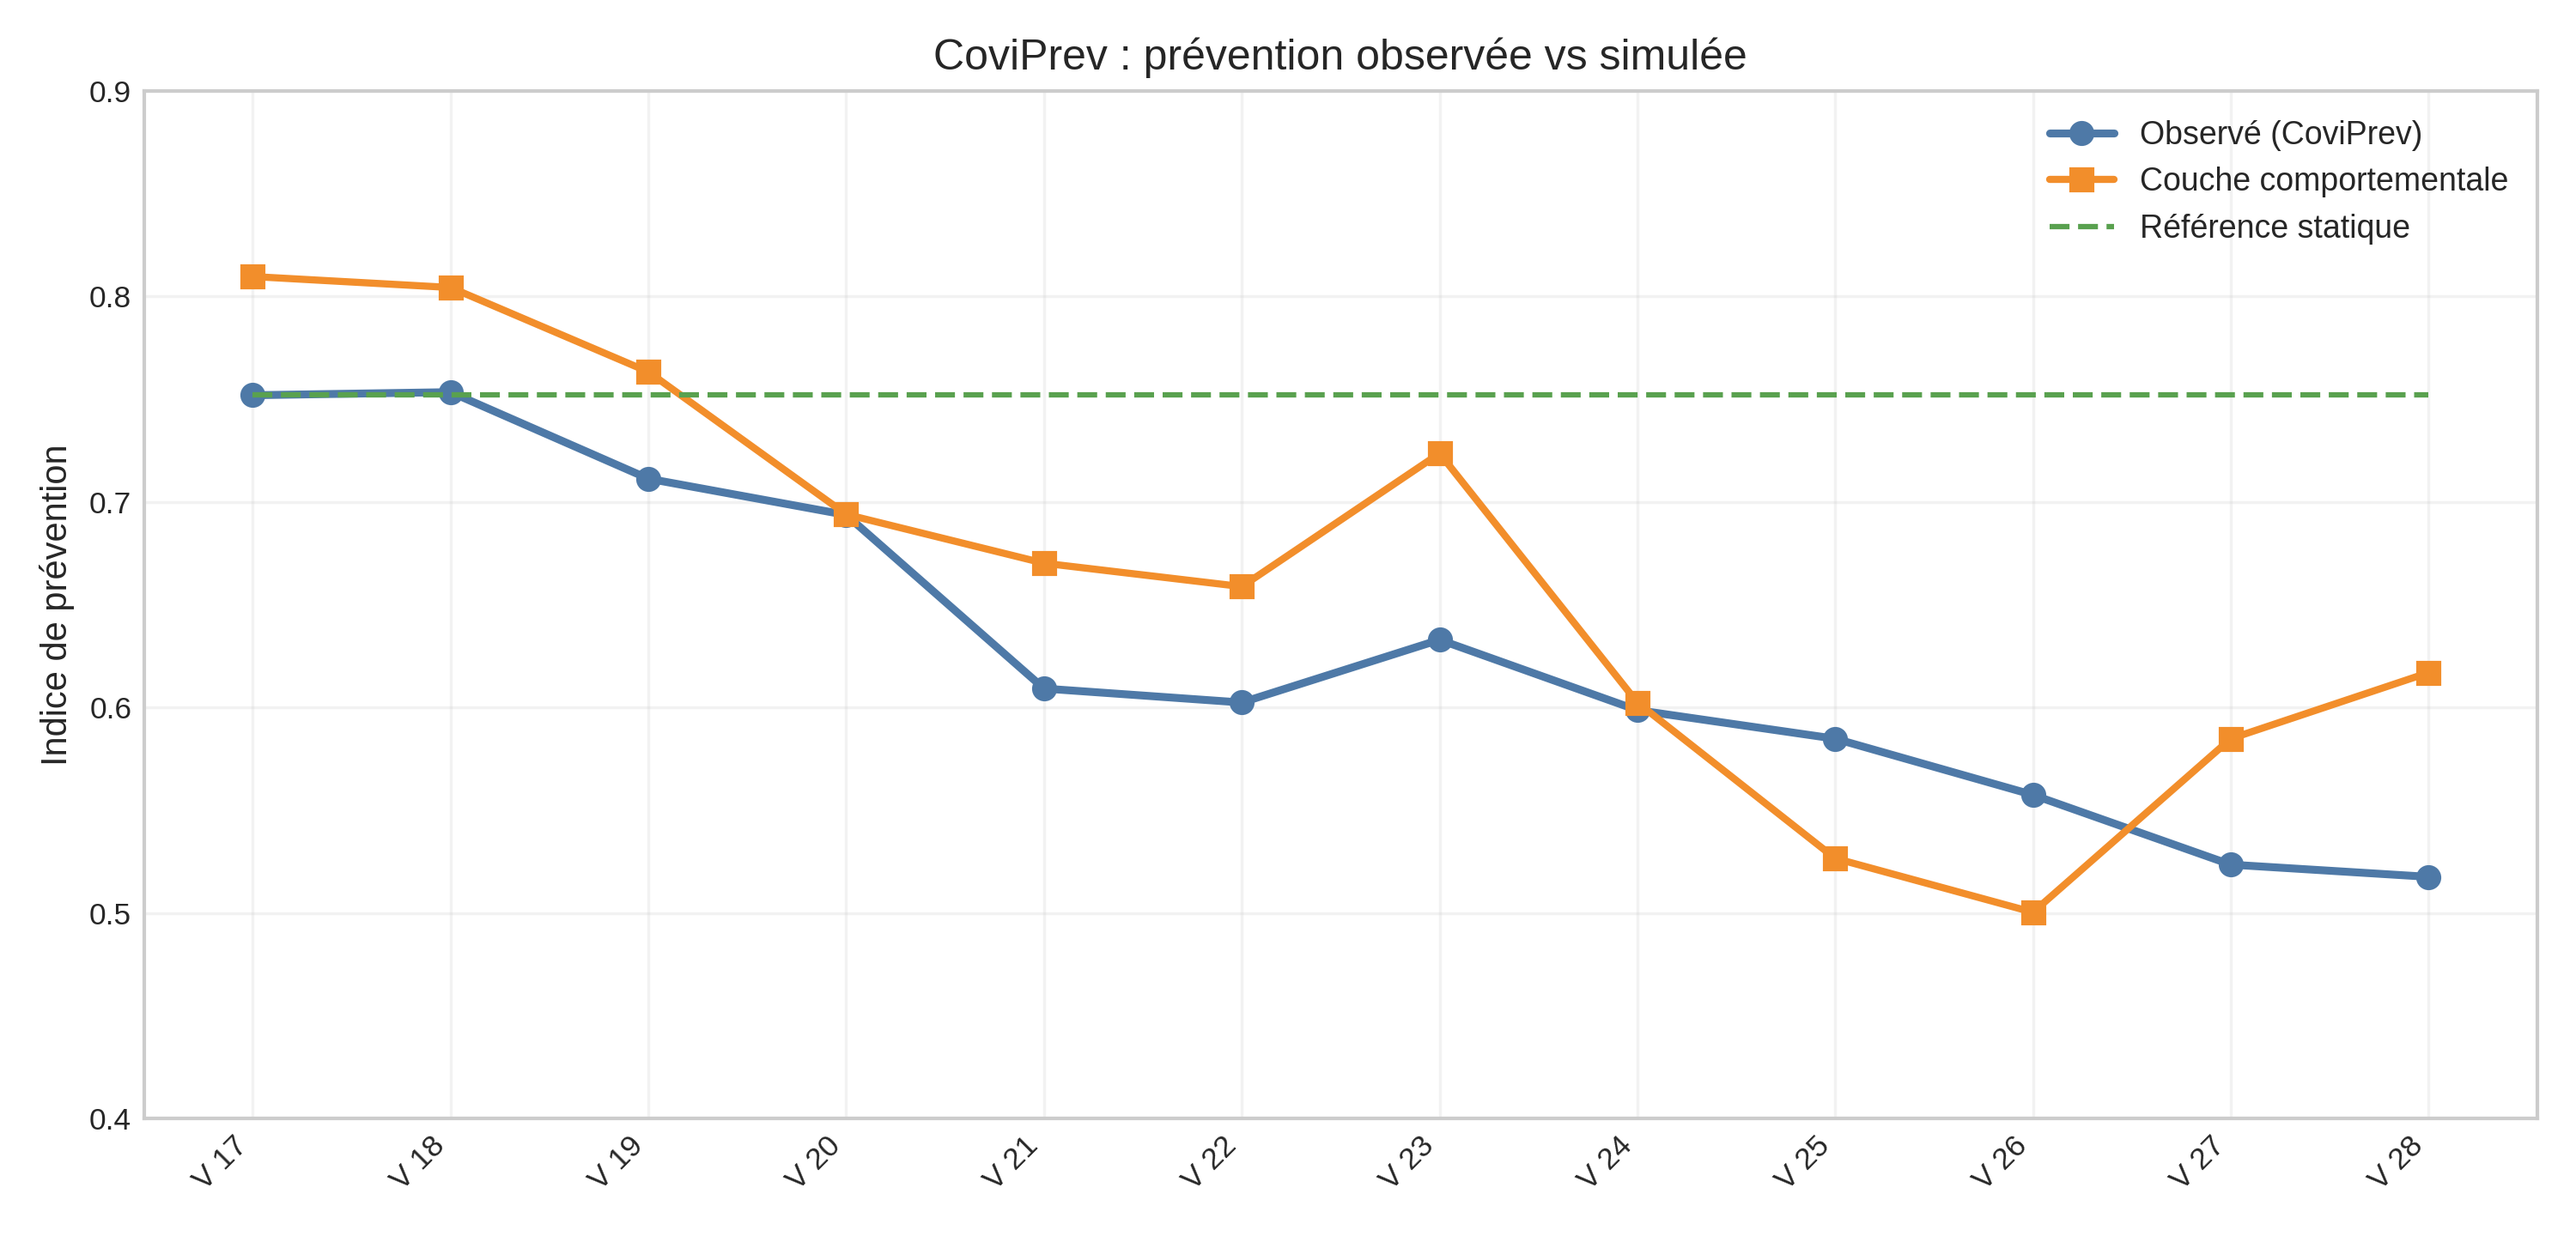
\includegraphics[width=0.92\textwidth]{figures/exp003_preventive_behavior_timeseries.png}
    \caption{Observed prevention index in CoviPrev and the corresponding simulation from the behavioral layer.}
    \label{fig:exp003-prevention}
\end{figure}

\begin{figure}[ht]
    \centering
    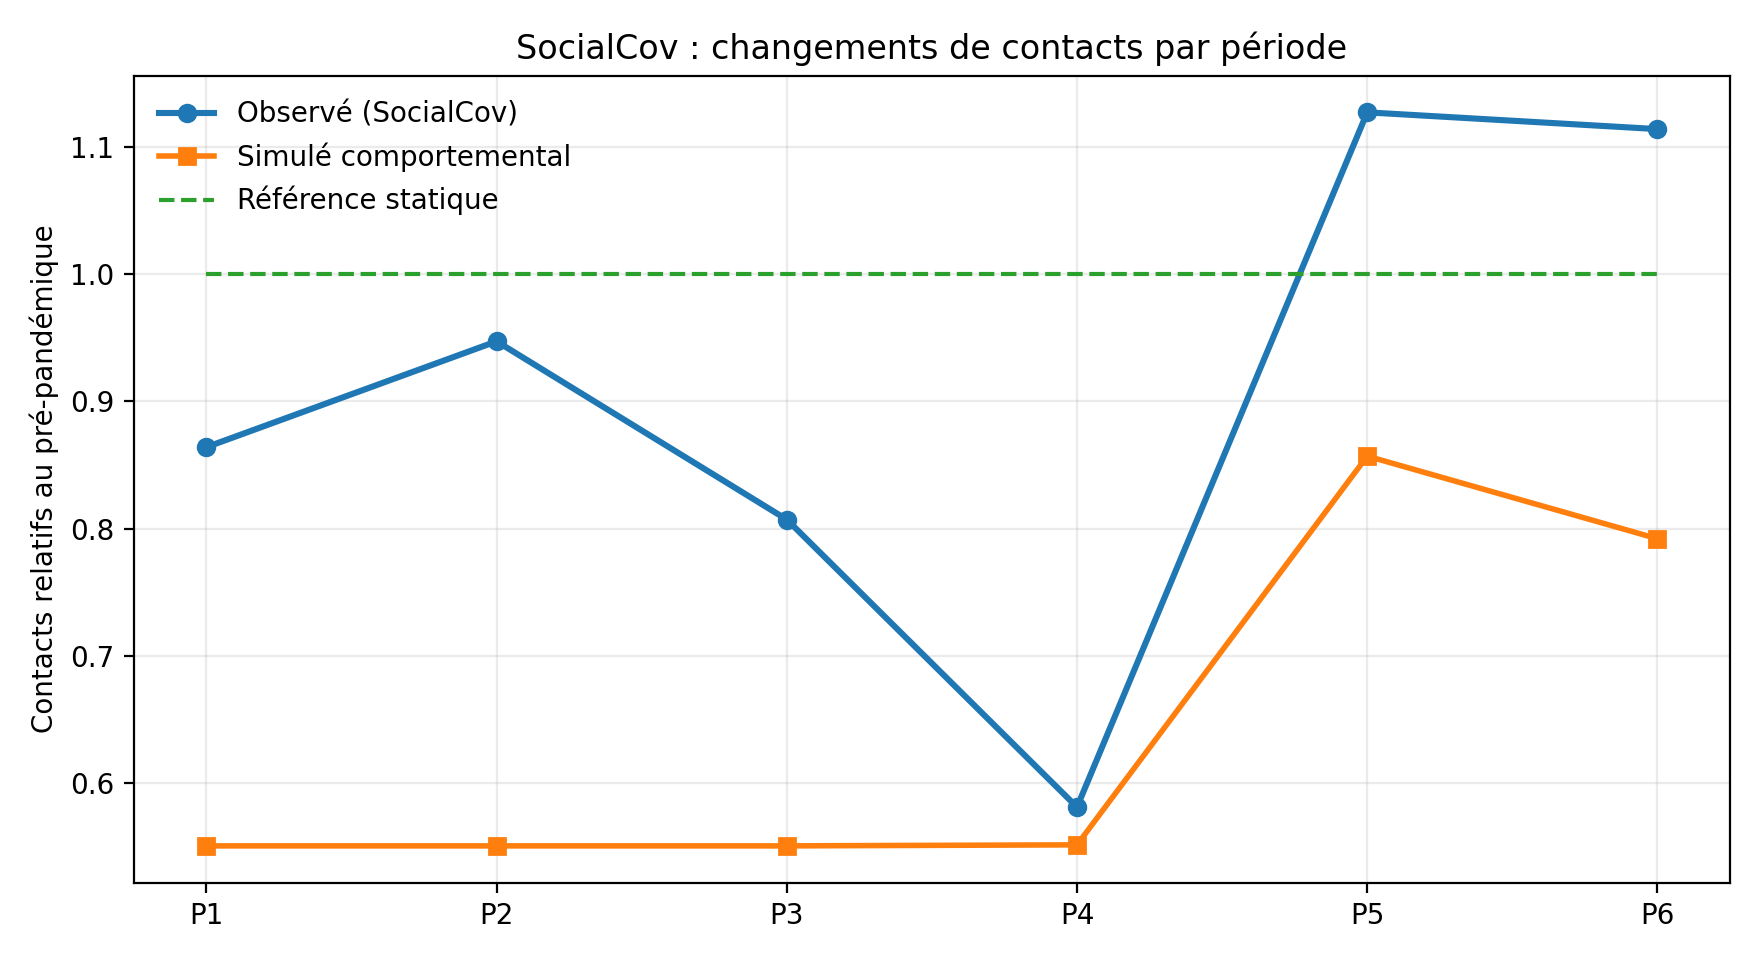
\includegraphics[width=0.88\textwidth]{figures/exp003_contact_changes_periods.png}
    \caption{Observed relative contact changes in SocialCov and the corresponding simulation from the behavioral layer.}
    \label{fig:exp003-contacts}
\end{figure}

\subsection{First central result: the LLM layer reveals legible social heterogeneity}
Experiment \texttt{exp006\_llm\_agents} is the first central result of the paper. Unlike the intermediate versions of the pipeline, the retained execution relies on real calls to Claude Sonnet 4.6, with 18 profiles, six public-policy regimes and 108 archived profile-regime pairs. The first result is a clear temporal gradient consistent with the public-health chronology: mean simulated mobility reduction rises from 0.09 in the pre-pandemic phase to 0.71 during the first lockdown, then falls to 0.40 during reopening before rising again to 0.50 during the second wave, 0.61 under curfew and 0.41 during the pass sanitaire period. Mean mask adherence follows a similarly plausible trajectory.

\begin{table}[ht]
    \centering
    \small
    \caption{Summary of aggregated LLM outputs by policy regime for the first \texttt{exp006} campaign. The three numerical columns are bounded scores between 0 and 1.}
    \begin{tabularx}{\linewidth}{>{\raggedright\arraybackslash}X r r r}
        \toprule
        Regime & LLM mobility & Observed mobility & LLM mask use \\
        \midrule
        Pre-pandemic & 0.09 & 0.05 & 0.04 \\
        First lockdown & 0.71 & 0.63 & 0.56 \\
        Reopening & 0.40 & 0.18 & 0.69 \\
        Second wave & 0.50 & 0.29 & 0.79 \\
        Curfew & 0.61 & 0.27 & 0.80 \\
        Pass sanitaire & 0.41 & 0.06 & 0.74 \\
        \bottomrule
    \end{tabularx}
\end{table}

Taken in isolation, this first LLM block remains imperfect. Across only six regimes, the correlation between simulated mobility reduction and observed mobility is 0.826, with an MAE of 0.206. This is not fine-grained calibration. It is nevertheless already useful for social sciences and applied epidemiology: the model recovers the general ordering of public-health regimes and makes visible a socially differentiated capacity for adjustment.

The most interesting result indeed concerns the ranking of responsiveness across profiles. The contrast between the profile \emph{white-collar professional aged 35--49 living with partner and children} and the profile \emph{farmer aged 50--64 living with partner} is marked and socially interpretable. White-collar profiles combine remote-work capacity, digital flexibility and higher trust in measures. Agricultural or manual-worker profiles remain more constrained by in-person activity, continuity of work and reduced room for adjustment. Figures \ref{fig:exp006-mobility}, \ref{fig:exp006-ranking} and \ref{fig:exp006-bias} synthesize this double result: correct ordering of regimes, followed by explicit social differentiation.

\begin{figure}[ht]
    \centering
    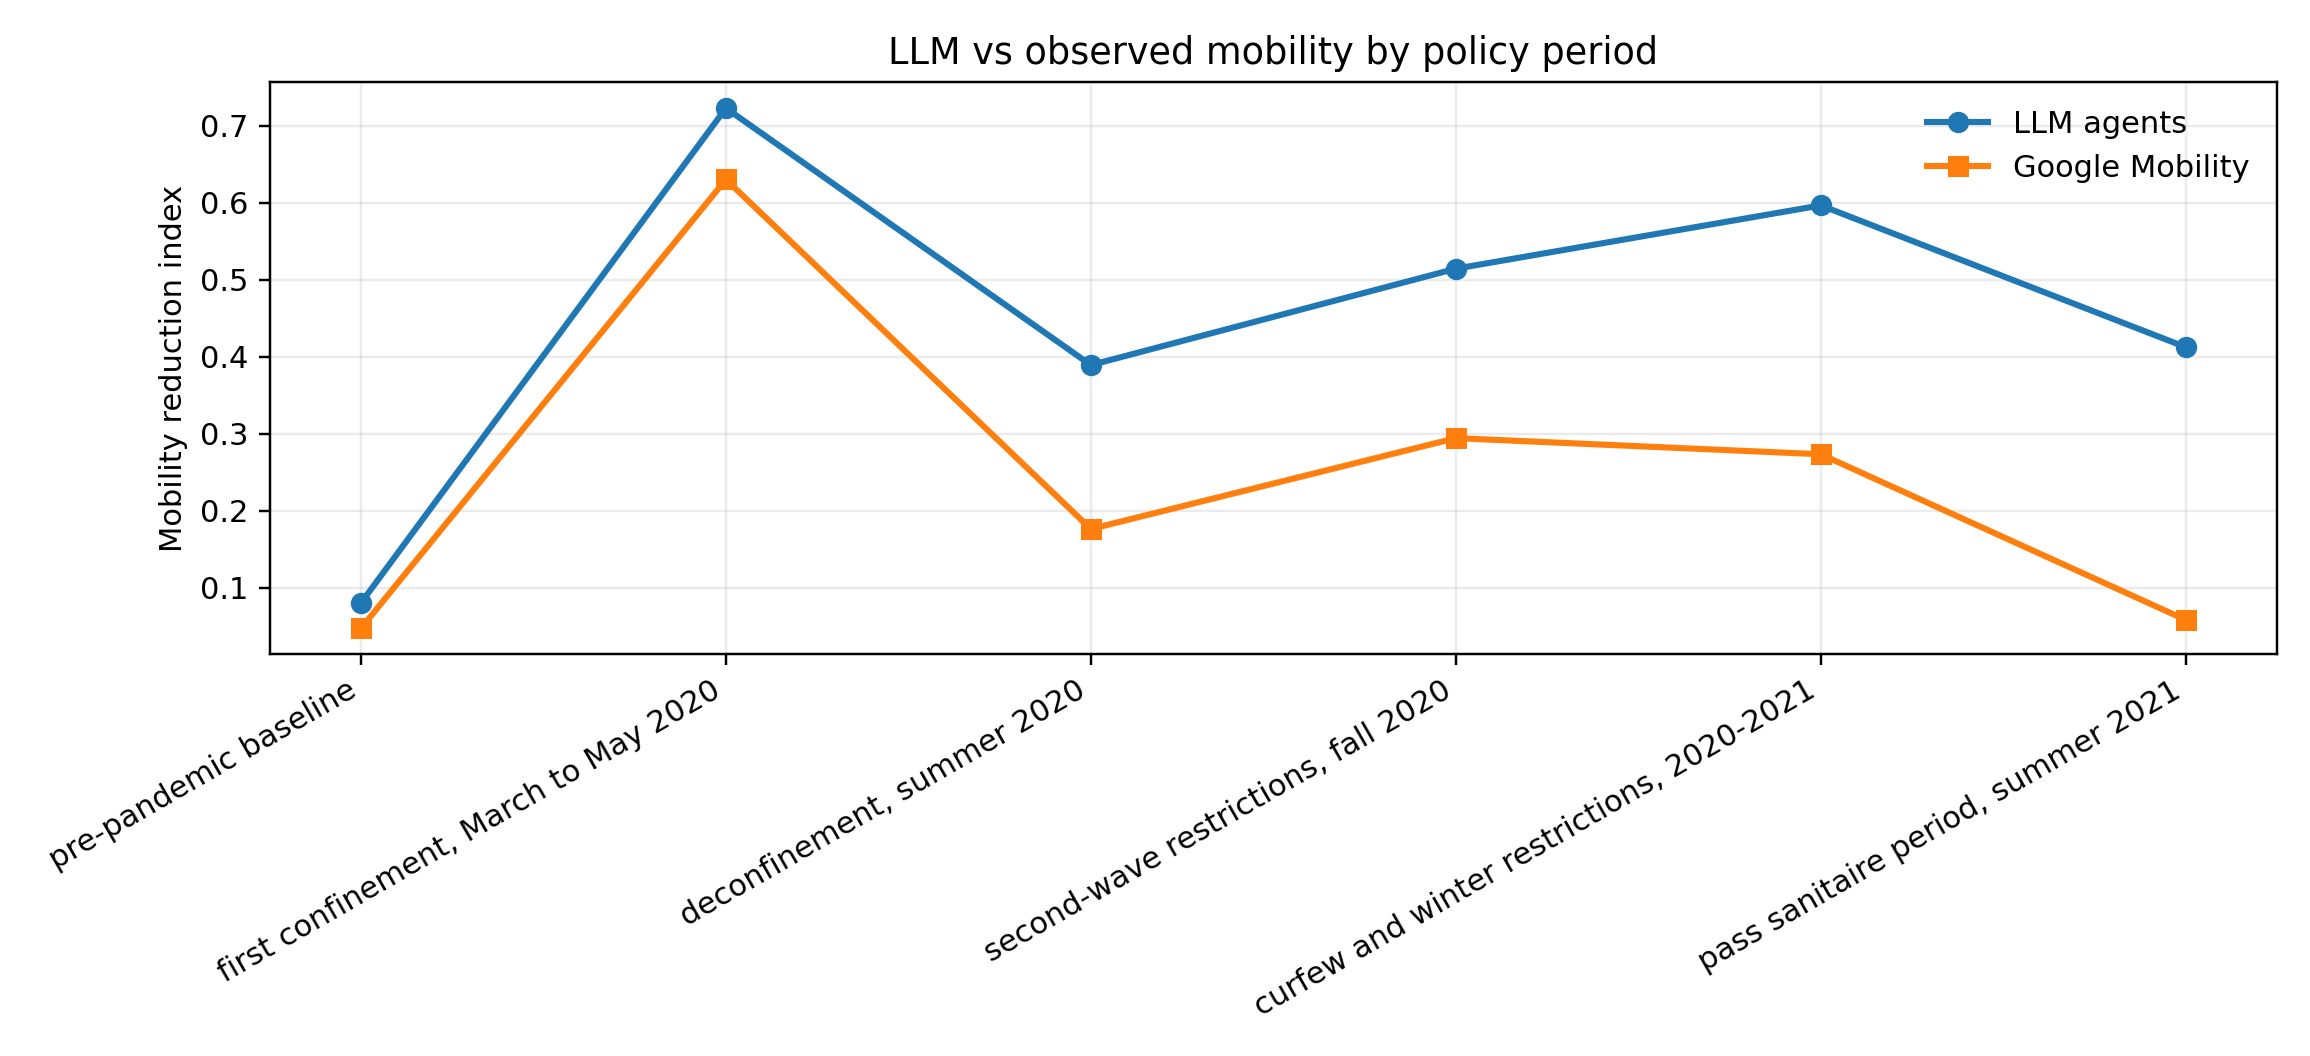
\includegraphics[width=0.92\textwidth]{figures/exp006_llm_vs_observed_mobility_by_policy.png}
    \caption{Aggregated mobility reduction from LLM agents, compared with the observed Google Mobility index, together with average mask adherence.}
    \label{fig:exp006-mobility}
\end{figure}

\begin{figure}[ht]
    \centering
    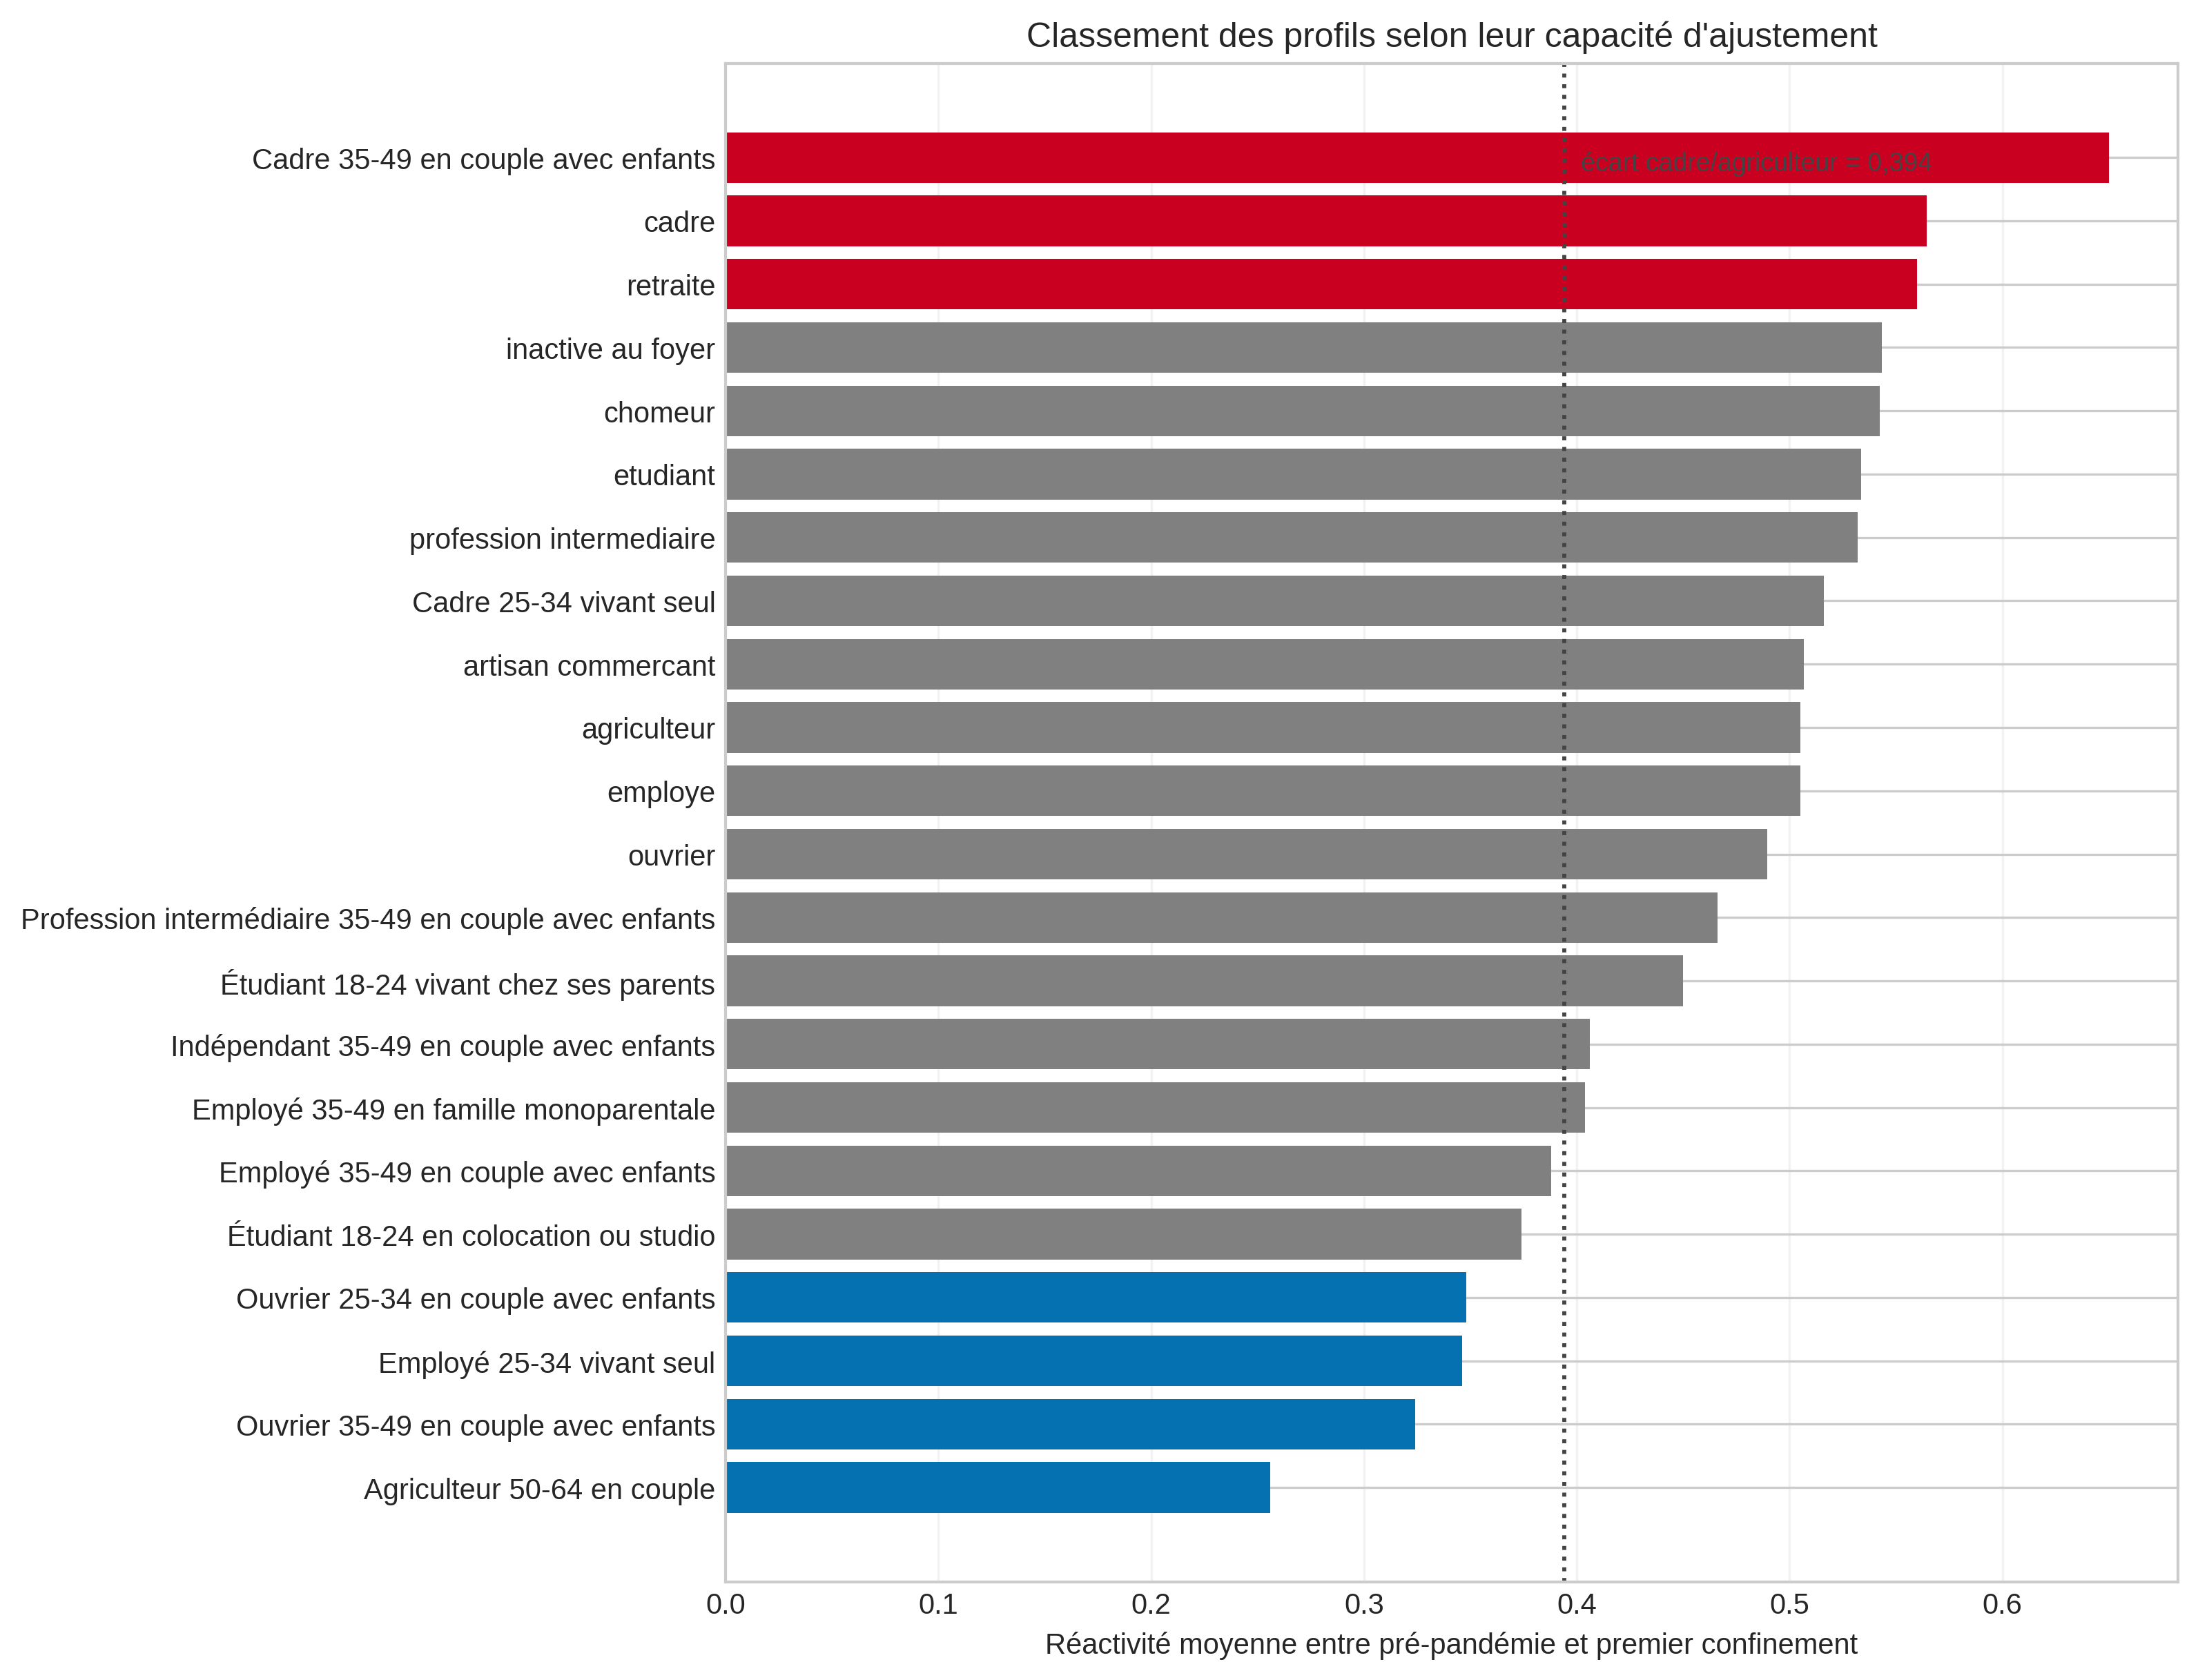
\includegraphics[width=0.92\textwidth]{figures/exp006_profile_responsiveness_ranking.png}
    \caption{Ranking of the 18 profiles according to their mean responsiveness between the pre-pandemic period and the first lockdown.}
    \label{fig:exp006-ranking}
\end{figure}

\begin{figure}[ht]
    \centering
    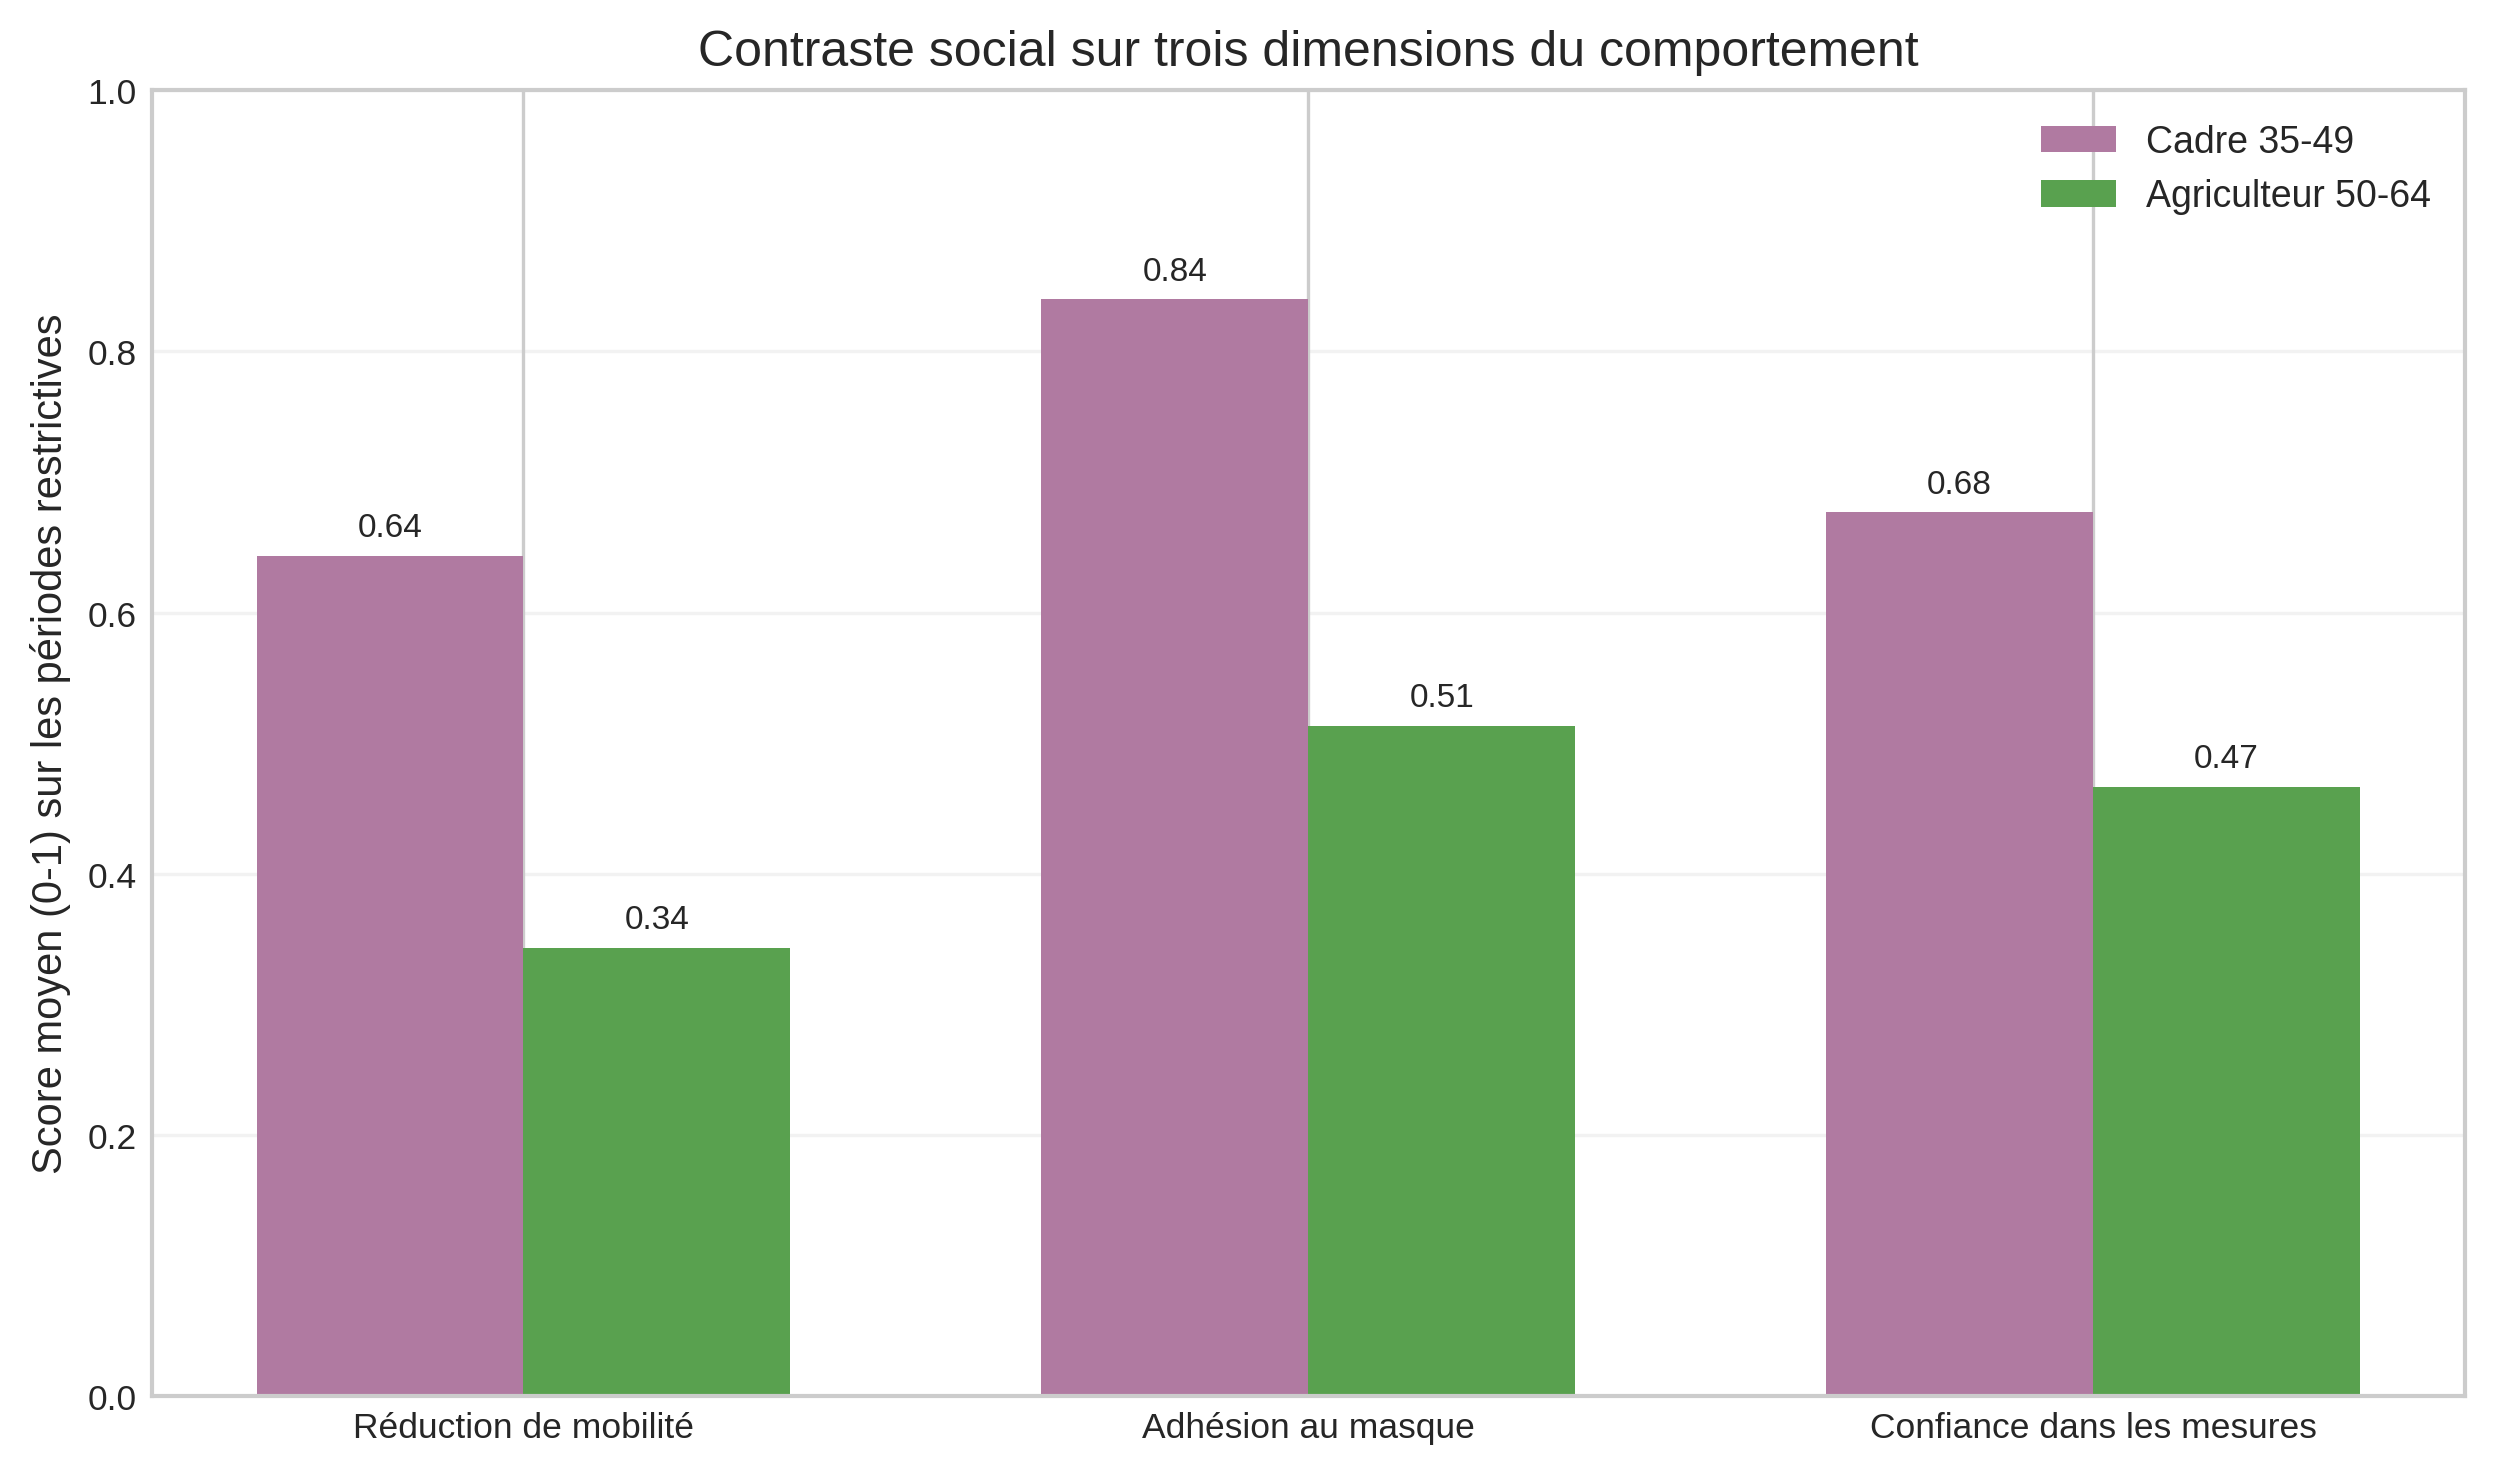
\includegraphics[width=0.78\textwidth]{figures/exp006_social_bias_analysis.png}
    \caption{Behavioral contrast between a white-collar profile and a farming profile during the most restrictive periods.}
    \label{fig:exp006-bias}
\end{figure}

\subsection{Main result: exp007 to exp009 turn the LLM block into a defensible SHS mediator}
The \texttt{exp007}, \texttt{exp008} and \texttt{exp009} sequence is the main result of this version of the paper. It should not be read as an implementation detail, but as a methodological experiment on how to integrate an LLM into the modeling chain. In \texttt{exp007}, the SHS mediator already produces a better prevention signal than the heuristic, with MAE 0.072 versus 0.141. Mobility, however, still fails clearly, with MAE 0.232 and correlation 0.851, against 0.094 and 0.863 for the heuristic baseline. The key observation is therefore asymmetric: the mediation idea works partly, but the latent mobility variable remains poorly framed.

\texttt{Exp008} then plays the role of a diagnostic experiment. By explicitly anchoring the mobility component, one obtains MAE 0.002 and a near-perfect correlation of 0.999. This experiment is not presented as a competing model, but as an analytical bound showing that the failure of \texttt{exp007} indeed comes from the specification of \emph{mobility\_reduction} rather than from any structural impossibility for the SHS/LLM layer to outperform the heuristic.

The final \texttt{exp009} campaign corrects that point directly. It preserves the SHS mediation logic, but replaces the initial protocol with a revised prompt centered on mobility and executes the final campaign on Claude Haiku 4.5. The result is substantially stronger: mobility MAE drops to 0.0219, versus 0.0935 for the heuristic, and mobility correlation rises to 0.989, versus 0.863 for the baseline. The prevention gain is maintained, with MAE 0.0685 versus 0.1409. The LLM block therefore does more than produce socially plausible profiles. In its final configuration, it becomes capable of outperforming the heuristic reference on two important aggregated dimensions.

\begin{table}[ht]
    \centering
    \footnotesize
    \caption{Progression of the SHS/LLM block across recent campaigns. Exp008 primarily serves as a diagnostic on mobility anchoring and is therefore not directly comparable on prevention.}
    \resizebox{\linewidth}{!}{%
    \begin{tabular}{llrrr}
        \toprule
        Campaign & Model & Mobility MAE & Mobility correlation & Prevention MAE \\
        \midrule
        Heuristic reference & Heuristic & 0.0935 & 0.863 & 0.1409 \\
        Initial Exp007 & Sonnet 4.6 & 0.2320 & 0.851 & 0.0724 \\
        Diagnostic Exp008 & Anchored & 0.0022 & 0.9998 & --- \\
        Final Exp009 & Haiku 4.5 & 0.0219 & 0.989 & 0.0685 \\
        \bottomrule
    \end{tabular}}
    \label{tab:llm-progression}
\end{table}

The meaning of this progression goes beyond numerical gain. It shows that the integration of LLMs into the study is not a cosmetic addition. The paper documents a methodical passage from a first campaign of plausible profiles, to a more ambitious mediation reformulation, to a localized partial failure, and then to a substantial correction that makes the central block scientifically defensible. That argumentative chain, more than any isolated score, is what gives the manuscript its coherence.

\section{Discussion}
The main conceptual change is the following: the center of the paper is no longer only the static baseline, but the way an SHS/LLM layer can be connected to it without losing readability. The static baseline remains important because it provides a transparent and robust anchor. The temporal layer retains descriptive value. But the most interesting result, at the interface between AI, social sciences and epidemiology, is the possibility of giving the LLM an explicit socio-behavioral mediation role rather than treating it as a mere generator of text or raw scores.

This framing brings the paper closer to the most cautious uses currently discussed in computational social science. Recent work shows that LLMs can become useful as annotation instruments, constrained simulation tools or hypothesis generators, provided that they remain embedded in explicit evaluation protocols and well-bounded tasks \citep{argyle2023out,park2023generative,horton2023homo,ziems2024css}. Our contribution now fits that line more clearly: the model is neither treated as a social oracle nor left free to generate the structure of the phenomenon on its own. It is mobilized as an additional mediation layer, grounded in named profiles, documented historical regimes and non-LLM controls.

The exp006 to exp009 sequence also clarifies a broader methodological point. An LLM block should not be evaluated as if it were a monolithic module. Results depend strongly on the abstraction level of profiles, the chosen output variable, the prompt, the way that output is reinjected into the pipeline, and the model itself. From that perspective, the partial failure of \texttt{exp007} is as instructive as the success of \texttt{exp009}. It shows that poor framing of one latent variable can cancel part of the useful signal even when the general SHS structure is relevant. Conversely, the strong improvement of \texttt{exp009} indicates that much of the gain comes from the articulation between model, prompt and projection layer, not from a simple effect of model brand or scale.

The fact that the final campaign was obtained on Claude Haiku 4.5 is interesting in itself. It suggests that a lighter model can remain scientifically useful when inserted into a tightly constrained protocol with structured outputs, explicit profiles and comparison against non-LLM baselines. This point echoes a broader observation in recent literature: the scientific value of these models is often much more dependent on the task, elicitation protocol and validation frame than on any abstract hierarchy between models \citep{ziems2024css}. This opens a natural perspective for future work: testing other LLM families, comparing more systematically generalist and compact models, and then exploring fine-tuned or instruction-tuned variants on structured socio-behavioral outputs. In such a program, the issue is not only raw performance. It is also separating more clearly the effect of the model, the effect of the prompt, and the effect of the mediation layer itself.

This opening must nevertheless remain cautious. The simulator does not discover social essences. It rearranges hypotheses about class position, work, housing, trust and mobility constraint that we explicitly encoded, and that the language model then reorganizes. The white-collar versus farming contrast, which is highly visible in the outputs, is therefore interesting because it makes the distributive assumptions of the pipeline audible and contestable. It should not be naturalized as a definitive measurement of French social groups. This caution is fully aligned with the literature warning against stereotyping and over-interpretation in large language models \citep{weidinger2022taxonomy,bender2021stochastic}.

Taken together, the contribution of the paper can now be stated more clearly. We do not propose either a substitute for French surveys or a full social simulation. We show that it is possible to insert an audited SHS/LLM layer into a French contact-matrix pipeline, compare it against explicit controls, and obtain a final version that is strong enough to beat a heuristic on aggregated mobility and prevention. The result remains bounded, but it becomes more interesting: it is no longer only a paper about a good baseline, but a paper about the conditions under which integrating LLMs into an epidemiological study can become methodologically credible.

\section{Limitations}
The first limitation is the most obvious one: the static baseline remains aggregated into 17 age classes and a single national matrix. This representation erases important heterogeneities, whether territorial, intra-household, calendar-based or occupational. It is suitable for a control-oriented protocol, but it would become insufficient for localized policies or fine-grained scenarios.

A second limitation concerns the temporal layer. Despite real gains on the prevention index, out-of-sample results remain fragile on SocialCov, and some simple ablations improve test MAE further. The dynamic part of the pipeline therefore remains more demonstrative than mature.

A third limitation concerns the status of the SHS profiles. The 18 profile-situations are analytical objects built from public margins, INSEE sources, remote-work proxies and reasoned behavioral indices. They are useful for making assumptions discussable, but they do not constitute individual observations. Differences across profiles should be read as structured scenarios, not as direct estimates by socio-professional category.

A fourth limitation concerns external validation of the LLM block. The targets used for prevention and profile alignment remain partial, because public data do not provide complete and homogeneous PCS-stratified measurement for all relevant dimensions. The paper therefore mainly demonstrates aggregated coherence and internal coherence of outputs rather than strong profile-by-profile validation against observed behavior.

A fifth limitation is specific to the exp007 to exp009 sequence. The final result of \texttt{exp009} is strong, but it does not settle the issue of model choice. Only a small number of LLM families are compared here, and the observed improvement combines both a change in prompt protocol and a change of model. It would therefore be premature to conclude that one specific model structurally dominates another. The next reasonable step is precisely to factor this experimental plan into a multi-model benchmark and prompt ablations, then, if the pattern holds, into fine-tuned variants on structured socio-behavioral outputs. This is also the direction recommended by recent computational social-science literature, which emphasizes comparative evaluation over ad hoc demonstration \citep{ziems2024css}.

A sixth limitation affects network reproducibility of the LLM block. Archived outputs make it possible to reproduce exactly the retained tables and figures, but online regeneration depends on a configured access environment and on provider-side generation that is not strictly seeded. Traceability of artefacts is good. Replication of the raw generation step remains weaker than for purely deterministic blocks.

Finally, the overall evaluation still relies on a limited number of metrics. MAE, Frobenius distance, correlation, local assortativity and directional agreement provide a useful but partial reading. Stronger claims would require additional criteria, for example downstream impact on an epidemic simulator, sensitivity to another age binning, or robustness to systematic perturbations of profiles and policy regimes.

\section{Conclusion}
The manuscript now yields a clearer reading of the project. The optimized static baseline on COMES-F remains useful and scientifically solid. The temporal layer brings an informative perspective on selected French series while remaining fragile out of sample. But the central contribution of the paper lies in the integration of an explicit, progressive and audited SHS/LLM layer within a French contact-matrix pipeline.

This point matters because it does not rest on a single spectacular isolated result. It rests on a readable experimental trajectory. A first campaign on Claude Sonnet 4.6 shows that a profiled LLM can already recover a plausible ordering of public-health regimes and socially differentiated responsiveness. A second sequence, exp007 to exp009, identifies the main bottleneck, corrects it, and ends in a final configuration on Claude Haiku 4.5 that outperforms the heuristic on both aggregated mobility and prevention. The most useful result is therefore not only a better score. It is the demonstration that an LLM layer can become methodologically credible if it is bounded, compared, diagnosed and reinjected cleanly into a modeling framework.

From that perspective, the paper should not be read as a promise to replace surveys, nor as proof of strong behavioral validity. It should be read as a proposal of method: how to connect named social profiles, public-policy regimes and epidemiologically relevant contact modifiers while keeping every assumption visible. That transparency, even more than raw performance, is what makes the article useful today and what opens the logical next steps of the project toward multi-LLM comparison, more systematic protocols and, eventually, fine-tuned models on structured socio-behavioral outputs.

% Auto-generated English companion table for the ROIA manuscript
{\tiny
\setlength{\LTleft}{0pt}
\setlength{\LTright}{0pt}
\renewcommand{\arraystretch}{1.03}
\begin{longtable}{@{}>{\raggedright\arraybackslash}p{0.17\linewidth}>{\raggedright\arraybackslash}p{0.43\linewidth}ccc@{}}
\caption{Socio-demographic profiles used in experiment Exp006. The \texttt{trust\_proxy}, preventive multiplier and mobility constraint columns are synthetic parameters bounded between 0 and 1.}\label{tab:profiles}\\
\toprule
Key & Synthetic description & Trust & Prevention & Mobility \\
\midrule
\endfirsthead
\toprule
Key & Synthetic description & Trust & Prevention & Mobility \\
\midrule
\endhead
\midrule
\multicolumn{5}{r}{\emph{Continued on next page}}\\
\endfoot
\bottomrule
\endlastfoot
\path{etudiant_18_24_parents} & Student aged 18--24 living with parents (student, parents' home) & 0.50 & 0.97 & 0.46 \\
\path{etudiant_18_24_colocation} & Student aged 18--24 in shared housing or studio (student, shared housing or studio) & 0.47 & 0.95 & 0.50 \\
\path{employe_25_34_seul} & Employee aged 25--34 living alone (employee, alone) & 0.49 & 0.99 & 0.74 \\
\path{employe_35_49_monoparent} & Employee aged 35--49 in a single-parent household (employee, single-parent household) & 0.46 & 0.98 & 0.78 \\
\path{ouvrier_25_34_couple_enfants} & Manual worker aged 25--34 living with partner and children (manual worker, couple with children) & 0.43 & 0.96 & 0.84 \\
\path{ouvrier_35_49_couple_enfants} & Manual worker aged 35--49 living with partner and children (manual worker, couple with children) & 0.41 & 0.96 & 0.85 \\
\path{employe_35_49_couple_enfants} & Employee aged 35--49 living with partner and children (employee, couple with children) & 0.50 & 1.00 & 0.72 \\
\path{profession_intermediaire_35_49_couple_enfants} & Intermediate profession aged 35--49 living with partner and children (intermediate profession, couple with children) & 0.58 & 1.02 & 0.58 \\
\path{cadre_25_34_seul} & White-collar professional aged 25--34 living alone (white-collar professional, alone) & 0.65 & 1.05 & 0.34 \\
\path{cadre_35_49_couple_enfants} & White-collar professional aged 35--49 living with partner and children (white-collar professional, couple with children) & 0.68 & 1.06 & 0.38 \\
\path{independant_35_49_couple_enfants} & Self-employed person aged 35--49 living with partner and children (craft or shop owner, couple with children) & 0.42 & 0.95 & 0.70 \\
\path{agriculteur_50_64_couple} & Farmer aged 50--64 living with partner (farmer, couple) & 0.48 & 0.98 & 0.72 \\
\path{inactif_50_64_seul} & Inactive adult aged 50--64 living alone (inactive adult at home, alone) & 0.51 & 1.01 & 0.44 \\
\path{chomeur_25_49_seul} & Unemployed adult aged 25--49 living alone or hosted by relatives (unemployed, alone or hosted) & 0.39 & 0.94 & 0.40 \\
\path{retraite_65_74_couple} & Retired adult aged 65--74 living with partner (retired, couple) & 0.64 & 1.08 & 0.42 \\
\path{retraite_75_plus_seul} & Retired adult aged 75+ living alone (retired, alone) & 0.66 & 1.10 & 0.34 \\
\path{employe_50_64_couple} & Employee aged 50--64 living with partner (employee, couple) & 0.54 & 1.03 & 0.66 \\
\path{ouvrier_50_64_couple} & Manual worker aged 50--64 living with partner (manual worker, couple) & 0.44 & 0.99 & 0.80 \\
\end{longtable}
}


\section*{Data and code availability}
All code, experiment configurations, JSON artefacts and figure-generation scripts are distributed publicly under the MIT License. External empirical data, especially COMES-F, CoviPrev, SocialCov and Google Community Mobility Reports, remain available through their original repositories and retain their respective licenses. The LLM campaigns retained in the manuscript are archived as structured JSON outputs, together with the aggregations and metadata required for exact reproduction of the retained tables and figures. Online regeneration of the LLM block nevertheless requires a configured environment and should not be confused with exact reproduction from archived artefacts.

\section*{Conflict of interest statement}
The author declares no conflict of interest related to this work. No remuneration was received from any organization likely to influence the conduct of the research or the writing of the manuscript.

\section*{Acknowledgements}
The author warmly thanks the teaching team of the University Diploma in Data Science at Université Paris 1 Panthéon-Sorbonne, which, despite organizational changes during the program, maintained careful and continuous support for the cohort. The author also thanks fellow students whose informal discussions helped sharpen several methodological directions of the project.

\bibliography{roia_manuscript}

\end{document}
